%utiliser les environnement \begin{comment} \end{comment} pour mettre en commentaire le préambule une fois la programmation appelée dans le document maître (!ne pas oublier de mettre en commentaire \end{document}!)

%--------------------------------------
%chap_A_addendeum_chimie_atomique
%--------------------------------------

\begin{comment}

\documentclass[a4paper, 11pt, twoside]{memoir}

\usepackage{AOCDTF}

%--------------------------------------
%CANEVAS
%--------------------------------------

\newcommand\BoxColor{\ifcase\thechapshift blue!30\or brown!30\or pink!30\or cyan!30\or green!30\or teal!30\or purple!30\or red!30\or olive!30\or orange!30\or lime!30\or gray!\or magenta!30\else yellow!30\fi} %définition de la couleur des marqueurs de chapitre

\newcounter{chapshift} %compteur de chapitre du marqueur de chapitre
\addtocounter{chapshift}{-1}
	
\newif\ifFrame %instruction conditionnelle pour les couleurs des pages
\Frametrue

\pagestyle{plain}

% the main command; the mandatory argument sets the color of the vertical box
\newcommand\ChapFrame{%
\AddEverypageHook{%
\ifFrame
\ifthenelse{\isodd{\value{page}}}
  {\backgroundsetup{contents={%
  \begin{tikzpicture}[overlay,remember picture]
  \node[
  	rounded corners=3pt,
    fill=\BoxColor,
    inner sep=0pt,
    rectangle,
    text width=1.5cm,
    text height=5.5cm,
    align=center,
    anchor=north west
  ] 
  at ($ (current page.north west) + (-0cm,-2*\thechapshift cm) $) %nombre négatif = espacement des marqueurs entre les différents chapitres (à régler en fin de rédaction) (4.5cm vaut un espacement équivalement à la hauteur du marqueur, une page peut en contenir 6 avec cet espacement-la mais il est le plus équilibré)
    {\rotatebox{90}{\hspace*{.5cm}%
      \parbox[c][1.2cm][t]{5cm}{%
        \raggedright\textcolor{black}{\sffamily\textbf{\leftmark}}}}};
  \end{tikzpicture}}}
  }
  {\backgroundsetup{contents={%
  \begin{tikzpicture}[overlay,remember picture]
  \node[
  	rounded corners=3pt,
    fill=\BoxColor,
    inner sep=0pt,
    rectangle,
    text width=1.5cm,
    text height=5.5cm,
    align=center,
    anchor=north east
  ] 
  at ($ (current page.north east) + (-0cm,-2*\thechapshift cm) $) %nombre négatif = espacement des marqueurs entre les différents chapitres (à régler en fin de rédaction) (4.5cm vaut un espacement équivalement à la hauteur du marqueur, une page peut en contenir 6 avec cet espacement-la mais il est le plus équilibré)
    {\rotatebox{90}{\hspace*{.5cm}%
      \parbox[c][1.2cm][t]{5cm}{%
        \raggedright\textcolor{black}{\sffamily\textbf{\leftmark}}}}};
  \end{tikzpicture}}}%
  }
  \BgMaterial%
  \fi%
}%
  \stepcounter{chapshift}
}

\renewcommand\chaptermark[1]{\markboth{\thechapter.~#1}{}} %redéfinition du marqueur de chapitre pour ne contenir que le titre du chapitre %à personnaliser selon le nombre de chapitre dans le cours

%--------------------------------------
%corps du document
%--------------------------------------

\begin{document} %corps du document
	\openleft %début de chapitre à gauche

\end{comment}

\chapter{Addendum de chimie atomique}
\label{ann:addendum_chimie_atomique}

Cet annexe regroupe tous les tableaux et figures mentionnés dans le \superref{chap:chimie_atomique} qui contiennent un nombre importants de données. Il n'est pas nécessaire de les retenir par c\oe{}ur mais ces informations constituent un support appréciable pour toute précision concernant ce chapitre.

%--------------------------------------
%PRE-REQUIS
%--------------------------------------

%utiliser les environnement \begin{comment} \end{comment} pour mettre en commentaire le préambule une fois la programmation appelée dans le document maître (!ne pas oublier de mettre en commentaire \end{document}!)

\documentclass[a4paper, 11pt, twoside, fleqn]{memoir}

\usepackage{AOCDTF}

%--------------------------------------
%CANEVAS
%--------------------------------------

\newcommand\BoxColor{\ifcase\thechapshift blue!30\or brown!30\or pink!30\or cyan!30\or green!30\or teal!30\or purple!30\or red!30\or olive!30\or orange!30\or lime!30\or gray!\or magenta!30\else yellow!30\fi} %définition de la couleur des marqueurs de chapitre

\newcounter{chapshift} %compteur de chapitre du marqueur de chapitre
\addtocounter{chapshift}{-1}
	
\newif\ifFrame %instruction conditionnelle pour les couleurs des pages
\Frametrue

\pagestyle{plain}

% the main command; the mandatory argument sets the color of the vertical box
\newcommand\ChapFrame{%
\AddEverypageHook{%
\ifFrame
\ifthenelse{\isodd{\value{page}}}
  {\backgroundsetup{contents={%
  \begin{tikzpicture}[overlay,remember picture]
  \node[
  	rounded corners=3pt,
    fill=\BoxColor,
    inner sep=0pt,
    rectangle,
    text width=1.5cm,
    text height=5.5cm,
    align=center,
    anchor=north west
  ] 
  at ($ (current page.north west) + (-0cm,-2*\thechapshift cm) $) %nombre négatif = espacement des marqueurs entre les différents chapitres (à régler en fin de rédaction) (4.5cm vaut un espacement équivalement à la hauteur du marqueur, une page peut en contenir 6 avec cet espacement-la mais il est le plus équilibré)
    {\rotatebox{90}{\hspace*{.5cm}%
      \parbox[c][1.2cm][t]{5cm}{%
        \raggedright\textcolor{black}{\sffamily\textbf{\leftmark}}}}};
  \end{tikzpicture}}}
  }
  {\backgroundsetup{contents={%
  \begin{tikzpicture}[overlay,remember picture]
  \node[
  	rounded corners=3pt,
    fill=\BoxColor,
    inner sep=0pt,
    rectangle,
    text width=1.5cm,
    text height=5.5cm,
    align=center,
    anchor=north east
  ] 
  at ($ (current page.north east) + (-0cm,-2*\thechapshift cm) $) %nombre négatif = espacement des marqueurs entre les différents chapitres (à régler en fin de rédaction) (4.5cm vaut un espacement équivalement à la hauteur du marqueur, une page peut en contenir 6 avec cet espacement-la mais il est le plus équilibré)
    {\rotatebox{90}{\hspace*{.5cm}%
      \parbox[c][1.2cm][t]{5cm}{%
        \raggedright\textcolor{black}{\sffamily\textbf{\leftmark}}}}};
  \end{tikzpicture}}}%
  }
  \BgMaterial%
  \fi%
}%
  \stepcounter{chapshift}
}

\renewcommand\chaptermark[1]{\markboth{\thechapter.~#1}{}} %redéfinition du marqueur de chapitre pour ne contenir que le titre du chapitre %à personnaliser selon le nombre de chapitre dans le cours

%--------------------------------------
%corps du document
%--------------------------------------

\begin{document} %corps du document
	\openleft %début de chapitre à gauche


\begin{table}[!h]
\begin{center}
\caption{Distribution des électrons dans les orbitales atomiques par sous-couche électronique\label{tab:exception_hund}\supercite{Wiki:TPE}}

\begin{threeparttable} %note dans tableau
\begin{tabularx}{\textwidth}{r c l X l @{\hspace{2cm}}X} \\ %tableau de plusieurs à 5 colonnes
\toprule %filet de haut de tableau
\multicolumn{3}{c}{\thead{\'Elément chimique}} & \thead[l]{Famille} & \multicolumn{2}{l}{\thead[l]{Configuration électronique}} \\
\midrule
$24$ 	& Cr 		& Chrome 			& Métal de transition 		& [Ar] 		& $\mathbf{4s^1 3d^5}$ \\
$28$ 	& Ni		& Nickel 			& Métal de transition 		& [Ar] 		& $\mathbf{4s^1 3d^9}$ \tnote{(*)} \\
$29$ 	& Cu		& Cuivre 			& Métal de transition 		& [Ar] 		& $\mathbf{4s^1 3d^{10}}$ \\
$41$ 	& Nb 	&Niobium 			& Métal de transition 		& [Kr] 		& $\mathbf{5s^1 4d^4}$ \\
$42$ 	& Mo 	& Molybdène 	& Métal de transition 		& [Kr] 		& $\mathbf{5s^1 4d^5}$ \\
$44$ 	&Ru 		& Ruthénium 	& Métal de transition 		& [Kr] 		& $\mathbf{5s^1 4d^7}$ \\
$45$		& Rh 	& Rhodium 		& Métal de transition	 	& [Kr] 		& $\mathbf{5s^1 4d^8}$ \\
$46$ 	& Pd 		& Palladium 		& Métal de transition 		& [Kr] 		& $\mathbf{4d^{10}}$ \\
$47$ 	& Ag 	& Argent 			& Métal de transition 		& [Kr] 		& $\mathbf{5s^1 4d^{10}}$ \\
$57$	 	& La 		& Lanthane 		& Lanthanide 				& [Xe] 		& $6s^2 \mathbf{5d^1}$ \\
$58$ 	& Ce 		& Cérium 			& Lanthanide 				& [Xe] 		& $6s^2 \mathbf{4f^1 5d^1}$ \\
$64$	 	& Gd 	& Gadolinium 	& Lanthanide 				& [Xe] 		& $6s^2 \mathbf{4f^7 5d^1}$ \\
$78$ 	& Pt 		& Platine 			& Métal de transition 		& [Xe] 		& $\mathbf{6s^1} 4f^14 \mathbf{5d^9}$ \\
$79$ 	& Au 	& Or 					& Métal de transition 		& [Xe] 		& $\mathbf{6s^1} 4f^{14} \mathbf{5d^{10}}$ \\
$89$  	& Ac 		& Actinium 		& Actinide 					& [Rn] 		& $7s^2 \mathbf{6d^1}$ \\
$90$ 	& 	Th 	& Thorium 		& Actinide 					& [Rn] 		& $7s^2 \mathbf{6d^2} $ \\
$91$ 	& Pa 		& Protactinium	& Actinide 					& [Rn] 		& $7s^2 \mathbf{5f^2 6d^1}$ \\
$92$		& U 		& Uranium 		& Actinide 					& [Rn] 		& $7s^2 \mathbf{5f^3 6d^1}$ \\
$96$ 	& Cm 	& Curium 			& Actinide 					& [Rn] 		& $7s^2 \mathbf{5f^7 6d^1}$ \\
$103$	& Lr 		& Lawrencium 	& Actinide 					& [Rn] 		& $7s^2 \mathbf{5f^{14} 7p^1}$ \\

\bottomrule

\end{tabularx}
\begin{tablenotes}
    \item[(*)] Le nickel présente deux configurations électroniques :
    \begin{compactitemize}
    		\item Une configuration régulière [Ar] $4s^2 3d^8$ présentant le niveau d'énergie le plus bas expérimentalement\,;
    		\item Une configuration irrégulière [Ar] $4s^1 3d^9$ présentant le niveau d'énergie moyen le plus bas. C'est cette configuration qui sera utilisée dans les calculs. 
	\end{compactitemize}
\end{tablenotes}
\end{threeparttable}
\end{center}
\end{table}

\end{document}

\begin{landscape}
	\begin{figure}
	\caption{Tableau périodique des éléments chimiques}
	\label{tab:tableau_periodique}
		\begin{center}
			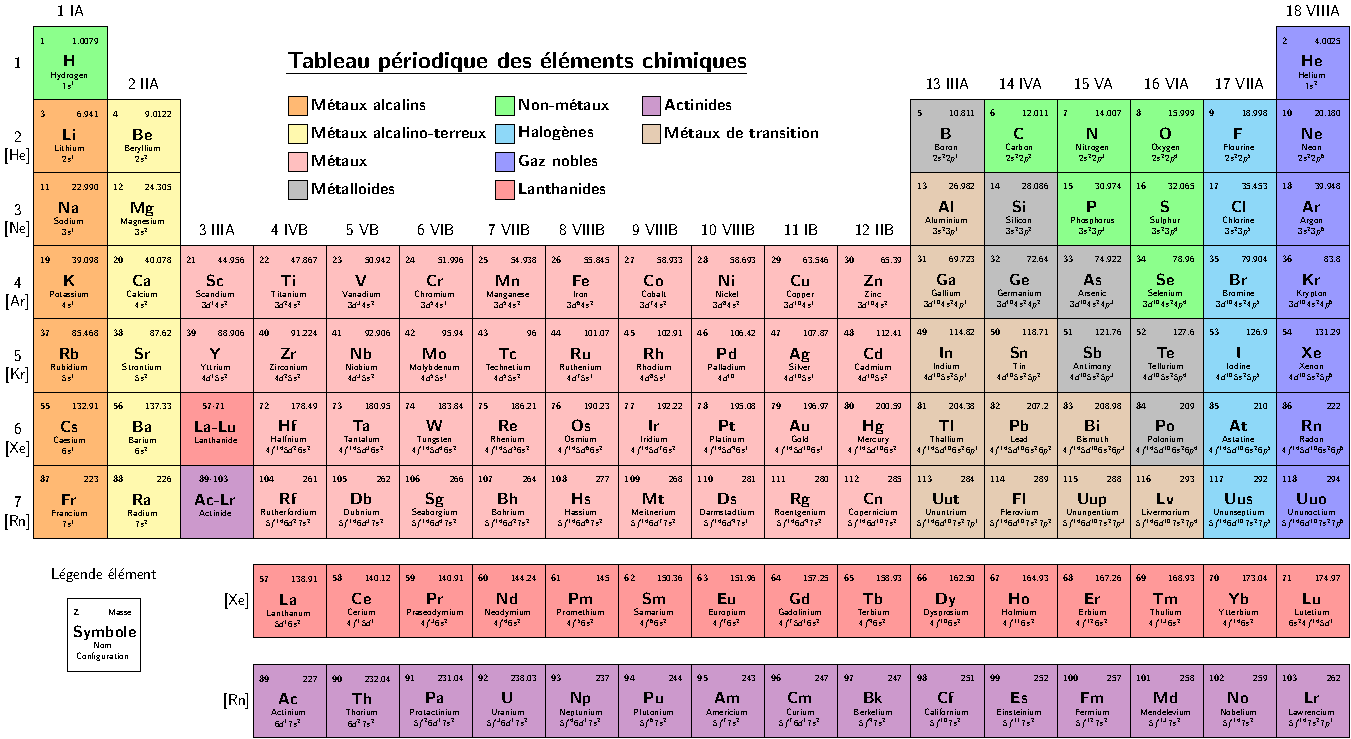
\includegraphics[scale=1.15]{tab_tableau_periodique.pdf} 
		\end{center}
	\end{figure}
\end{landscape}

%utiliser les environnement \begin{comment} \end{comment} pour mettre en commentaire le préambule une fois la programmation appelée dans le document maître (!ne pas oublier de mettre en commentaire \end{document}!)

\begin{comment}

\documentclass[a4paper, 11pt, twoside, fleqn]{memoir}

\usepackage{AOCDTF}

%--------------------------------------
%CANEVAS
%--------------------------------------

\newcommand\BoxColor{\ifcase\thechapshift blue!30\or brown!30\or pink!30\or cyan!30\or green!30\or teal!30\or purple!30\or red!30\or olive!30\or orange!30\or lime!30\or gray!\or magenta!30\else yellow!30\fi} %définition de la couleur des marqueurs de chapitre

\newcounter{chapshift} %compteur de chapitre du marqueur de chapitre
\addtocounter{chapshift}{-1}
	
\newif\ifFrame %instruction conditionnelle pour les couleurs des pages
\Frametrue

\pagestyle{plain}

% the main command; the mandatory argument sets the color of the vertical box
\newcommand\ChapFrame{%
\AddEverypageHook{%
\ifFrame
\ifthenelse{\isodd{\value{page}}}
  {\backgroundsetup{contents={%
  \begin{tikzpicture}[overlay,remember picture]
  \node[
  	rounded corners=3pt,
    fill=\BoxColor,
    inner sep=0pt,
    rectangle,
    text width=1.5cm,
    text height=5.5cm,
    align=center,
    anchor=north west
  ] 
  at ($ (current page.north west) + (-0cm,-2*\thechapshift cm) $) %nombre négatif = espacement des marqueurs entre les différents chapitres (à régler en fin de rédaction) (4.5cm vaut un espacement équivalement à la hauteur du marqueur, une page peut en contenir 6 avec cet espacement-la mais il est le plus équilibré)
    {\rotatebox{90}{\hspace*{.5cm}%
      \parbox[c][1.2cm][t]{5cm}{%
        \raggedright\textcolor{black}{\sffamily\textbf{\leftmark}}}}};
  \end{tikzpicture}}}
  }
  {\backgroundsetup{contents={%
  \begin{tikzpicture}[overlay,remember picture]
  \node[
  	rounded corners=3pt,
    fill=\BoxColor,
    inner sep=0pt,
    rectangle,
    text width=1.5cm,
    text height=5.5cm,
    align=center,
    anchor=north east
  ] 
  at ($ (current page.north east) + (-0cm,-2*\thechapshift cm) $) %nombre négatif = espacement des marqueurs entre les différents chapitres (à régler en fin de rédaction) (4.5cm vaut un espacement équivalement à la hauteur du marqueur, une page peut en contenir 6 avec cet espacement-la mais il est le plus équilibré)
    {\rotatebox{90}{\hspace*{.5cm}%
      \parbox[c][1.2cm][t]{5cm}{%
        \raggedright\textcolor{black}{\sffamily\textbf{\leftmark}}}}};
  \end{tikzpicture}}}%
  }
  \BgMaterial%
  \fi%
}%
  \stepcounter{chapshift}
}

\renewcommand\chaptermark[1]{\markboth{\thechapter.~#1}{}} %redéfinition du marqueur de chapitre pour ne contenir que le titre du chapitre %à personnaliser selon le nombre de chapitre dans le cours

%--------------------------------------
%corps du document
%--------------------------------------

\begin{document} %corps du document
	\openleft %début de chapitre à gauche

\end{comment}


\begin{landscape}
\begin{xltabular}{\linewidth}{C C C c c c c c c c}
\caption{Orbitales réelles d'un atome hydrogénoïde par triplet de nombres quantiques ($n, \ell, m_{\ell}$)\label{tab:geometrie_orbitale}\supercite{Wiki:OA}} 
\\
\toprule

\multicolumn{2}{c}{\thead{Nombre quantique}} & \multirow[c]{2}{*}{\thead{Sous-couche}} & \multicolumn{7}{c}{\thead{Module $\lvert M_\ell \rvert$ du nombre quantique magnétique}} \\

\cmidrule(lr){1-2} \cmidrule(lr){4-10} %filet de milieu de tableau centré sur les colonnes mentionnées

\thead{Principal} & \thead{Azimutal} & & \thead{$0$} & \multicolumn{2}{c}{\thead{$1$}} & \multicolumn{2}{c}{\thead{$2$}} & \multicolumn{2}{c}{\thead{$3$}} \\

\midrule %filet de milieu de tableau

\endfirsthead %en-tête de la première page du tableau  

\toprule

\multicolumn{2}{c}{\thead{Nombre quantique}} & \multirow[c]{2}{*}{\thead{Sous-couche}} & \multicolumn{7}{c}{\thead{Module $\lvert M_\ell \rvert$ du nombre quantique magnétique}} \\

\cmidrule(lr){1-2} \cmidrule(lr){4-10} %filet de milieu de tableau centré sur les colonnes mentionnées

\thead{Principal} & \thead{Azimutal} & & \thead{$0$} & \multicolumn{2}{c}{\thead{$1$}} & \multicolumn{2}{c}{\thead{$2$}} & \multicolumn{2}{c}{\thead{$3$}} \\

\midrule %filet de milieu de tableau

\endhead %en-tête de la première page du tableau
	\addlinespace
	\midrule %filet de milieu de tableau
	\multicolumn{10}{r}{\small\textit{Page suivante}}
\endfoot %pied de page de toutes les pages du tableau
\endlastfoot %pied de page de la dernièredu tableau

\multirow[t]{2}{*}{$n=1$} & \multirow[t]{2}{*}{$\ell=0$} & \multirow[t]{2}{*}{$1s$} & 
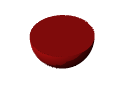
\includegraphics[width=1.6cm]{tableau_geometrie_orbitale_modelisation/S1M0.png} 

& & & & & & \\

& & & \makecell[c]{$1s$} & & & & & &  \\ %centrer la cellule individuellement horizontalement 

\midrule %filet de milieu de tableau

\multirow[t]{4}{*}{$n=2$} & \multirow[t]{2}{*}{$\ell=0$} & \multirow[t]{2}{*}{$2s$} & 
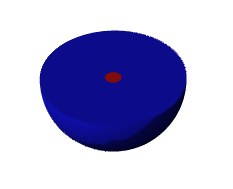
\includegraphics[width=1.6cm]{tableau_geometrie_orbitale_modelisation/S2M0.png} 
& & & & & & \\

& & & \makecell[c]{$2s$} & & & & & &  \\ %centrer la cellule individuellement 

\addlinespace

& \multirow[t]{2}{*}{$\ell=1$} & \multirow[t]{2}{*}{$2p$} & 
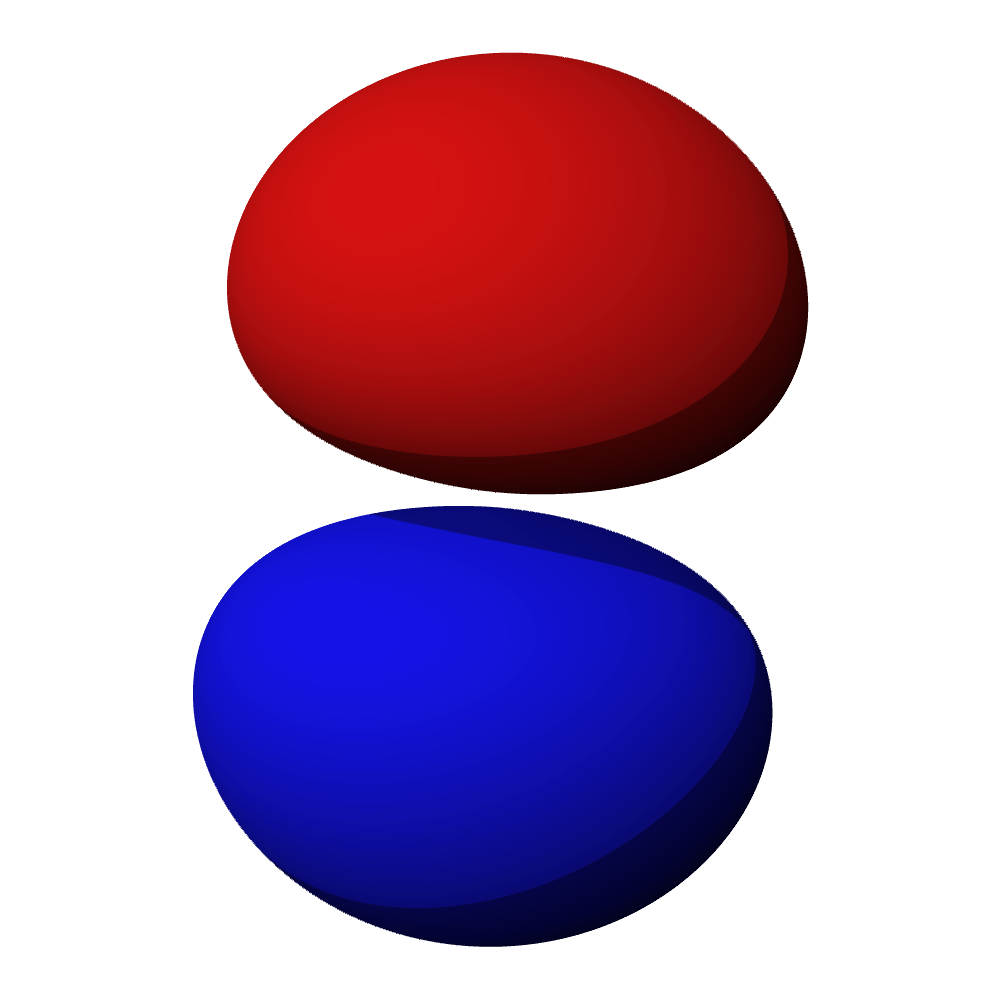
\includegraphics[width=1.6cm]{tableau_geometrie_orbitale_modelisation/Pz_orbital.png} 
&
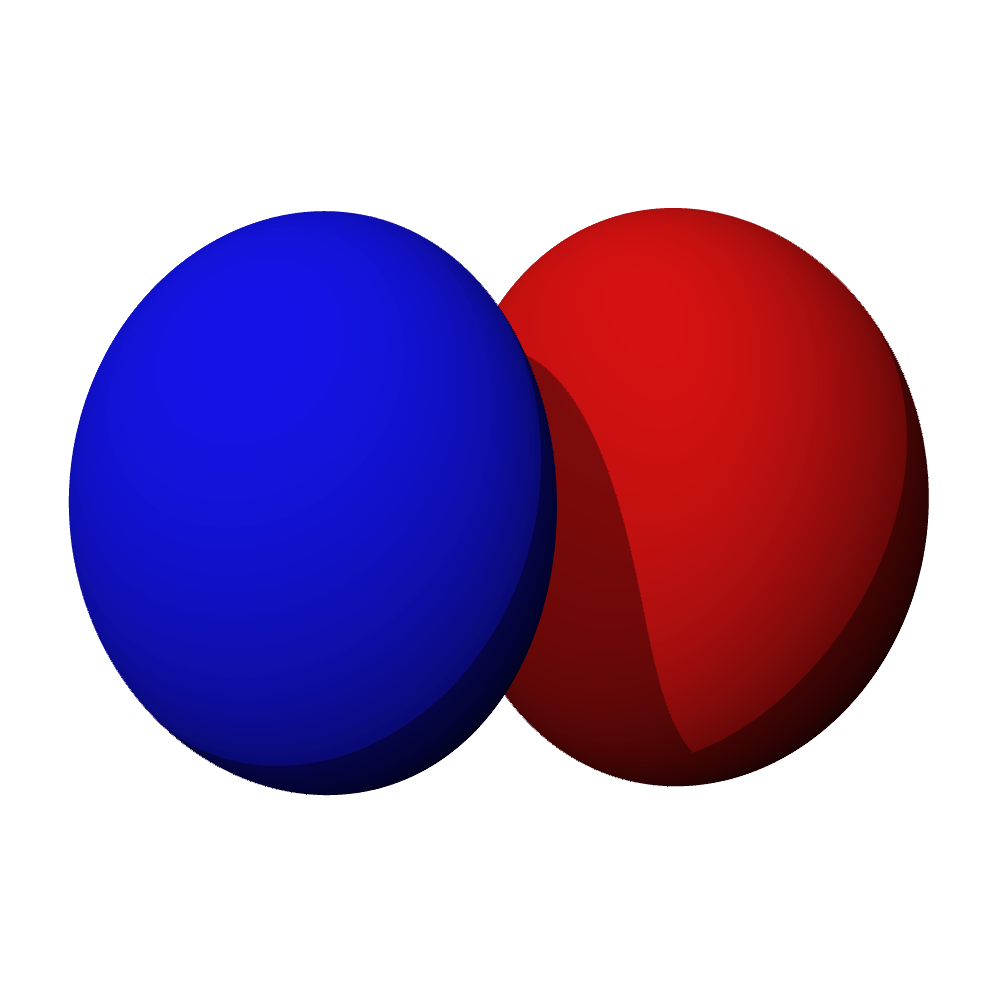
\includegraphics[width=1.6cm]{tableau_geometrie_orbitale_modelisation/Px_orbital.png}  
&
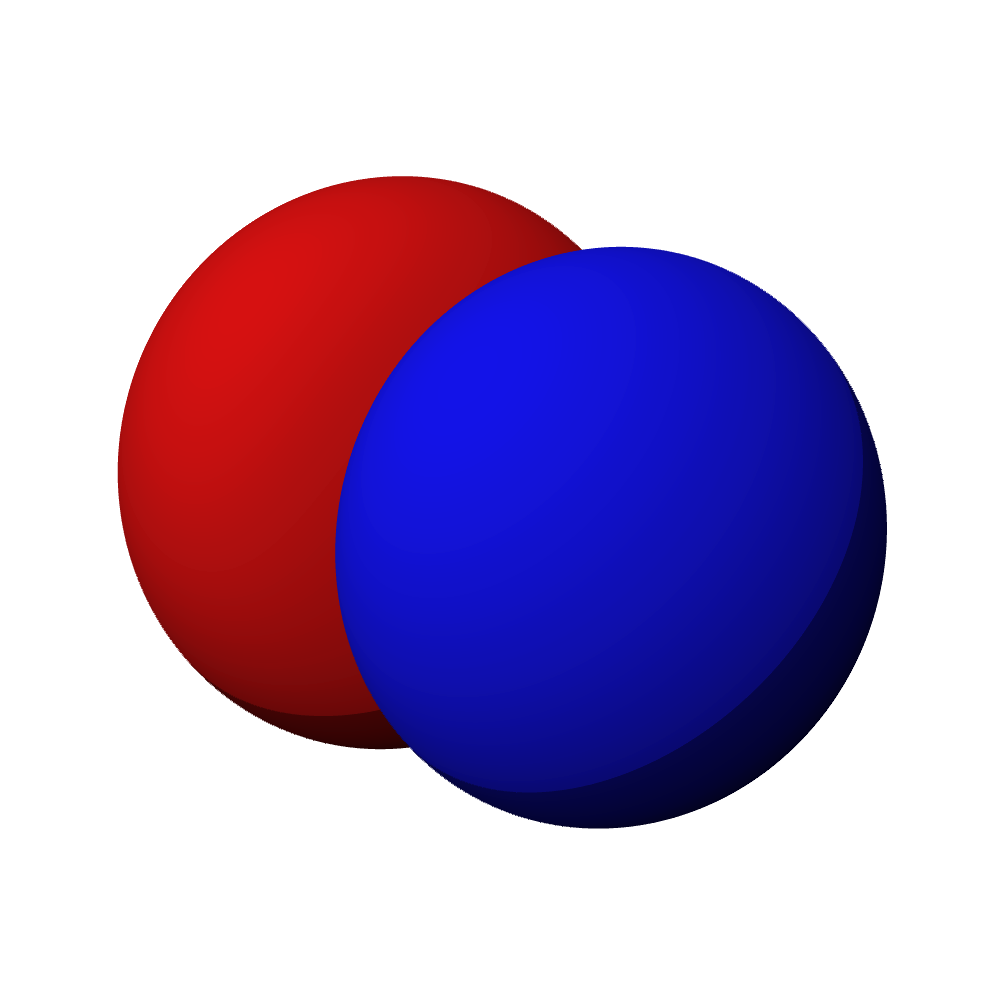
\includegraphics[width=1.6cm]{tableau_geometrie_orbitale_modelisation/Py_orbital.png} 
& & & & \\

& & & \makecell[c]{$2p_z$} & \makecell[c]{$2p_x$} & \makecell[c]{$2p_y$} & & & &  \\ %centrer la cellule individuellement 

\midrule %filet de milieu de tableau

\multirow[t]{6}{*}{$n=3$} & \multirow[t]{2}{*}{$\ell=0$} & \multirow[t]{2}{*}{$3s$} & 
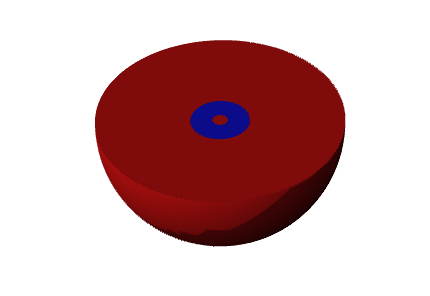
\includegraphics[width=1.6cm]{tableau_geometrie_orbitale_modelisation/S3M0.png} 
& & & & & & \\

& & & \makecell[c]{$3s$} & & & & & &  \\ %centrer la cellule individuellement 

\addlinespace

& \multirow[t]{2}{*}{$\ell=1$} & \multirow[t]{2}{*}{$3p$} & 
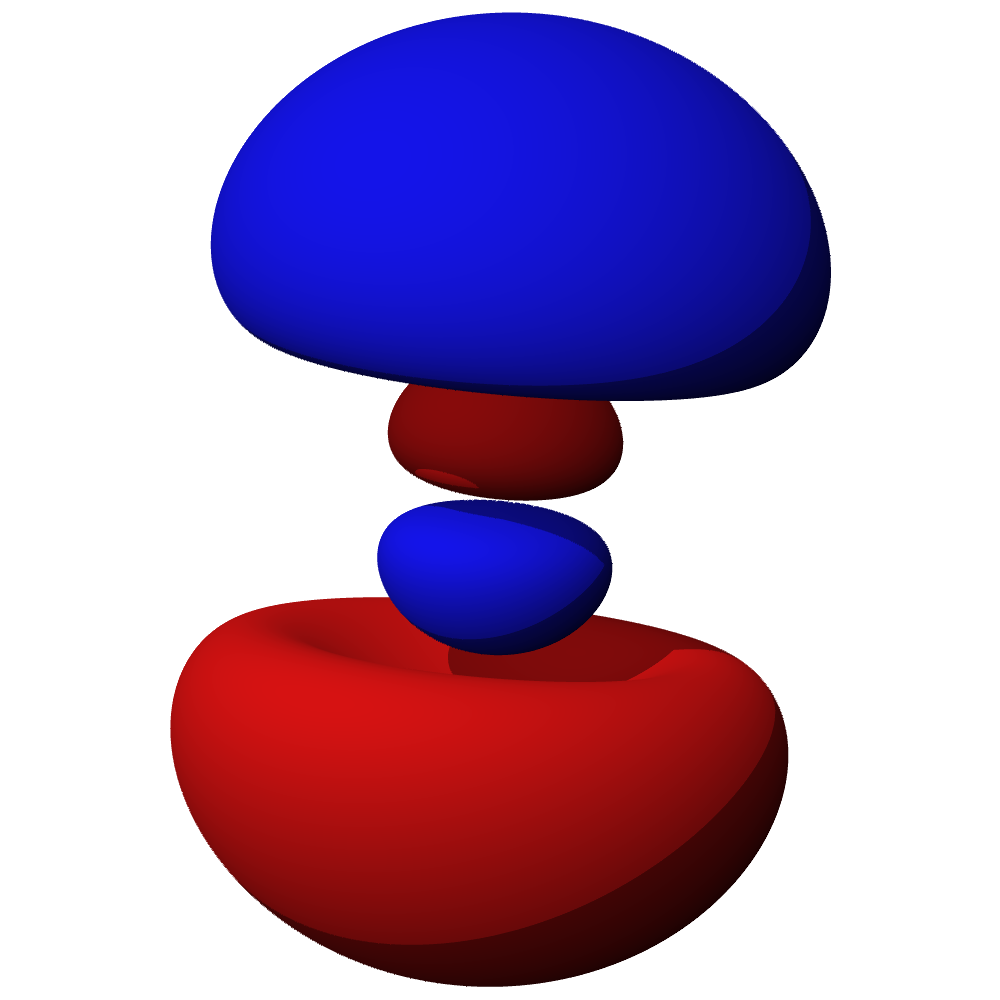
\includegraphics[width=1.6cm]{tableau_geometrie_orbitale_modelisation/P3z.png} 
&
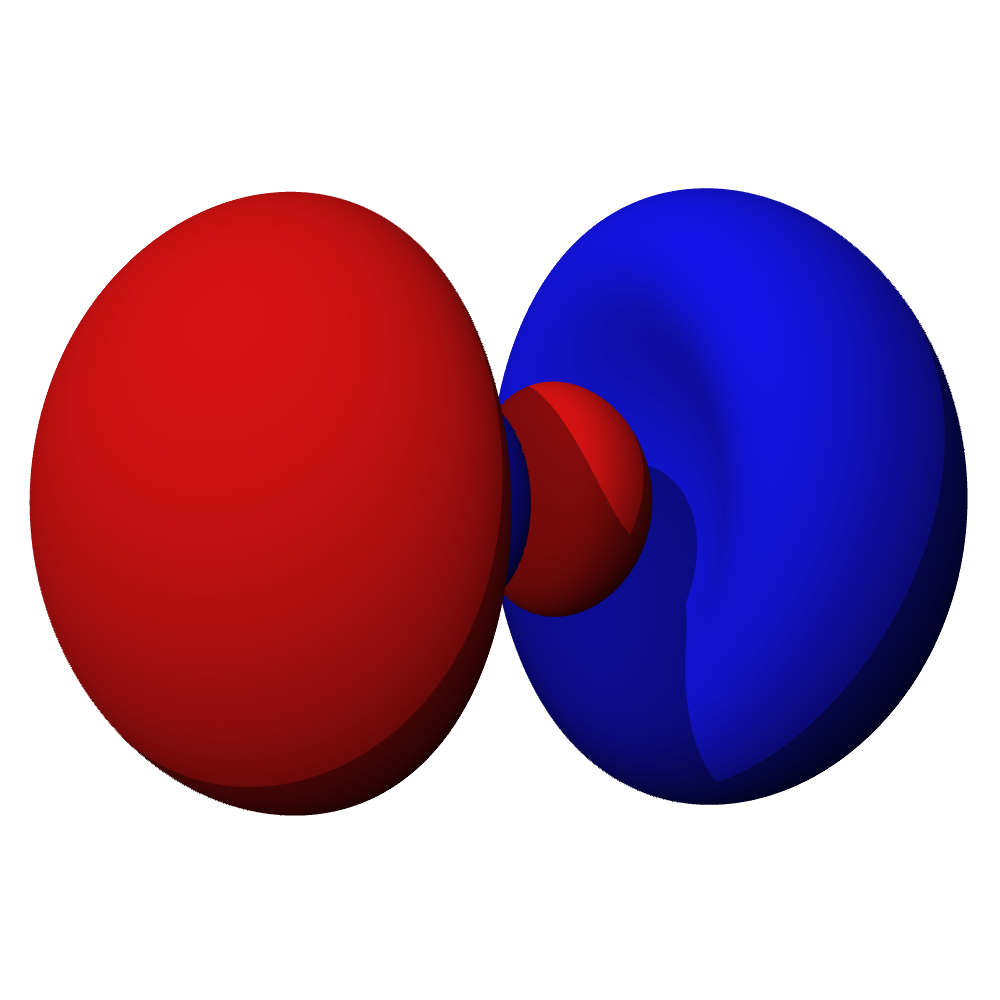
\includegraphics[width=1.6cm]{tableau_geometrie_orbitale_modelisation/P3x.png}  
&
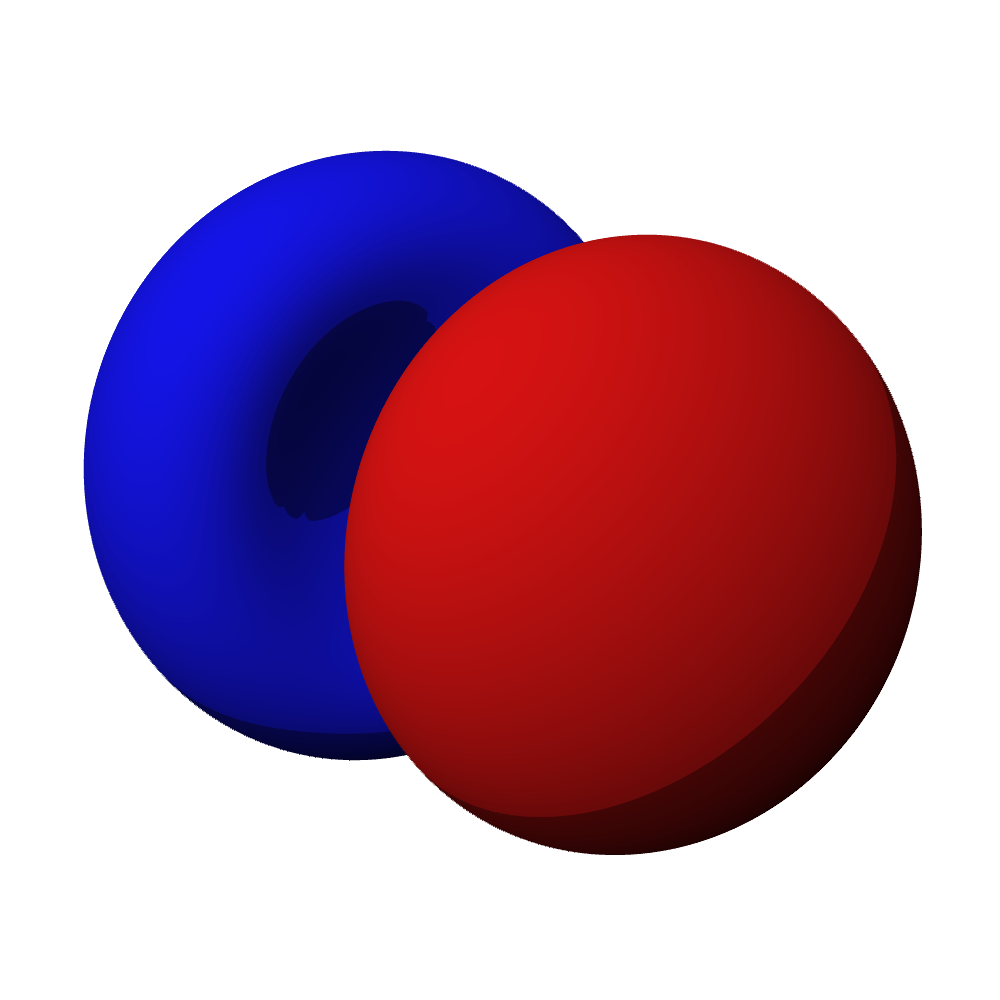
\includegraphics[width=1.6cm]{tableau_geometrie_orbitale_modelisation/P3y.png} 
& & & & \\

& & & \makecell[c]{$3p_z$} & \makecell[c]{$3p_x$} & \makecell[c]{$3p_y$} & & & &  \\ %centrer la cellule individuellement 

\addlinespace

 & \multirow[t]{2}{*}{$\ell=2$} & \multirow[t]{2}{*}{$3d$} & 
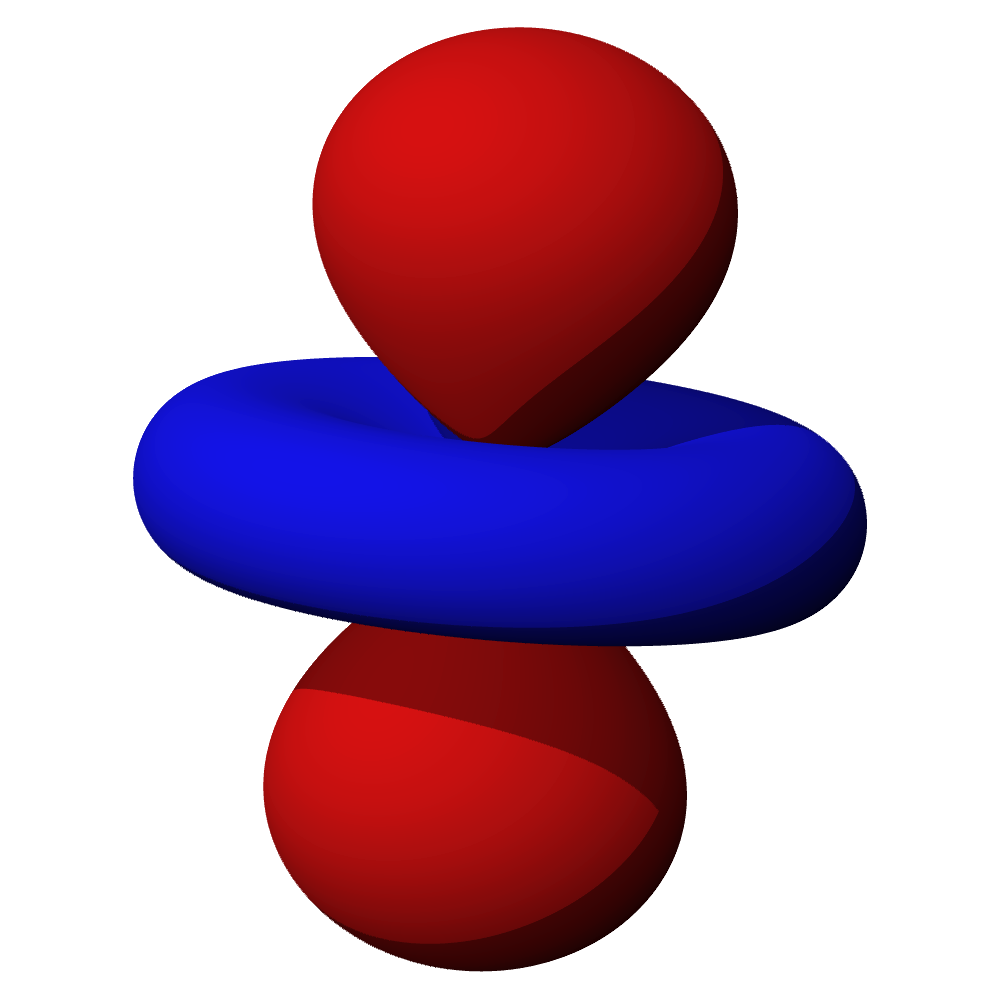
\includegraphics[width=1.6cm]{tableau_geometrie_orbitale_modelisation/Dz2_orbital.png} 
&
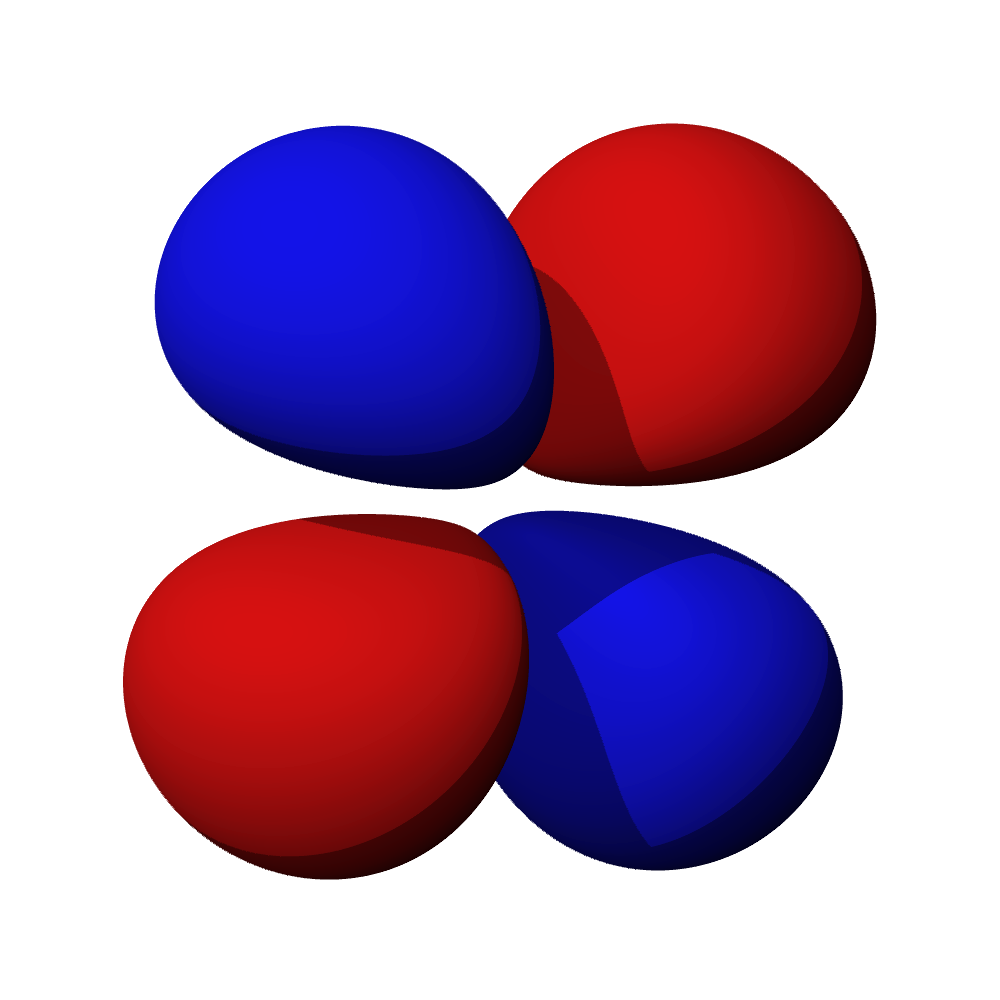
\includegraphics[width=1.6cm]{tableau_geometrie_orbitale_modelisation/Dxz_orbital.png}  
&
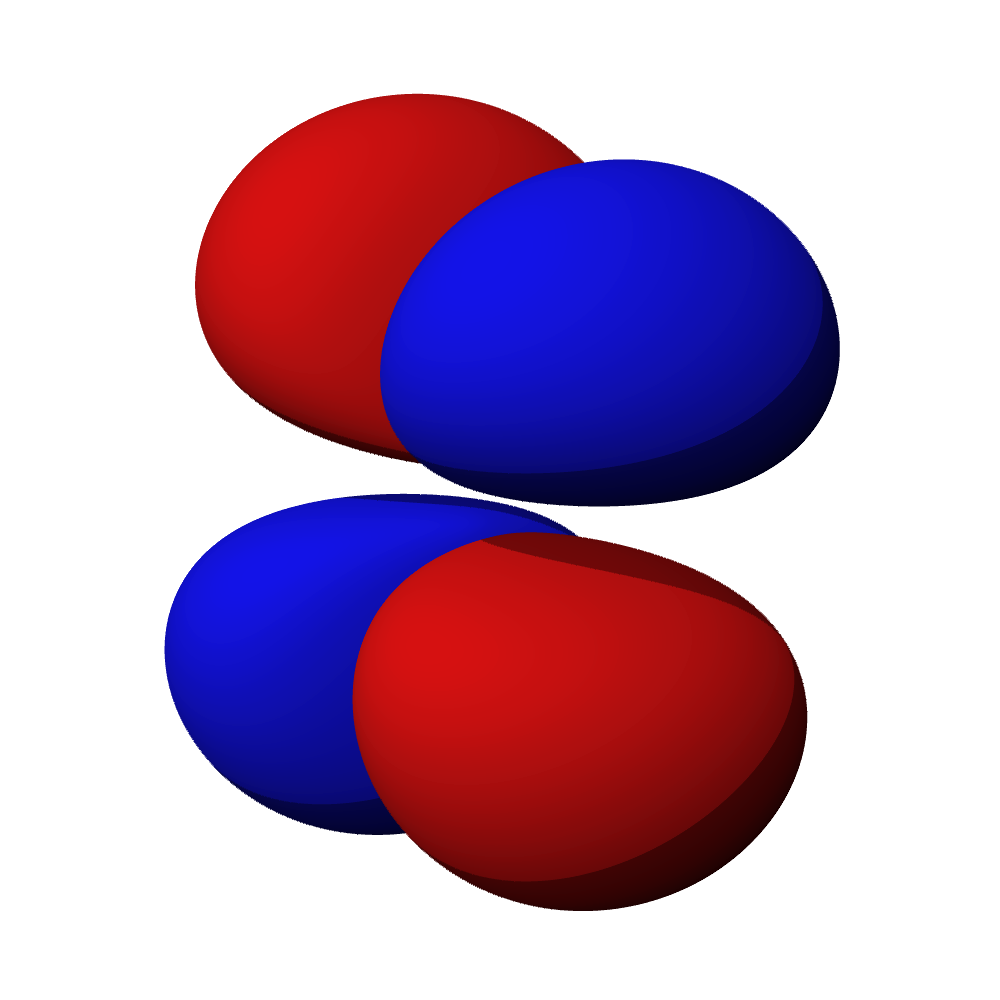
\includegraphics[width=1.6cm]{tableau_geometrie_orbitale_modelisation/Dyz_orbital.png} 
& 
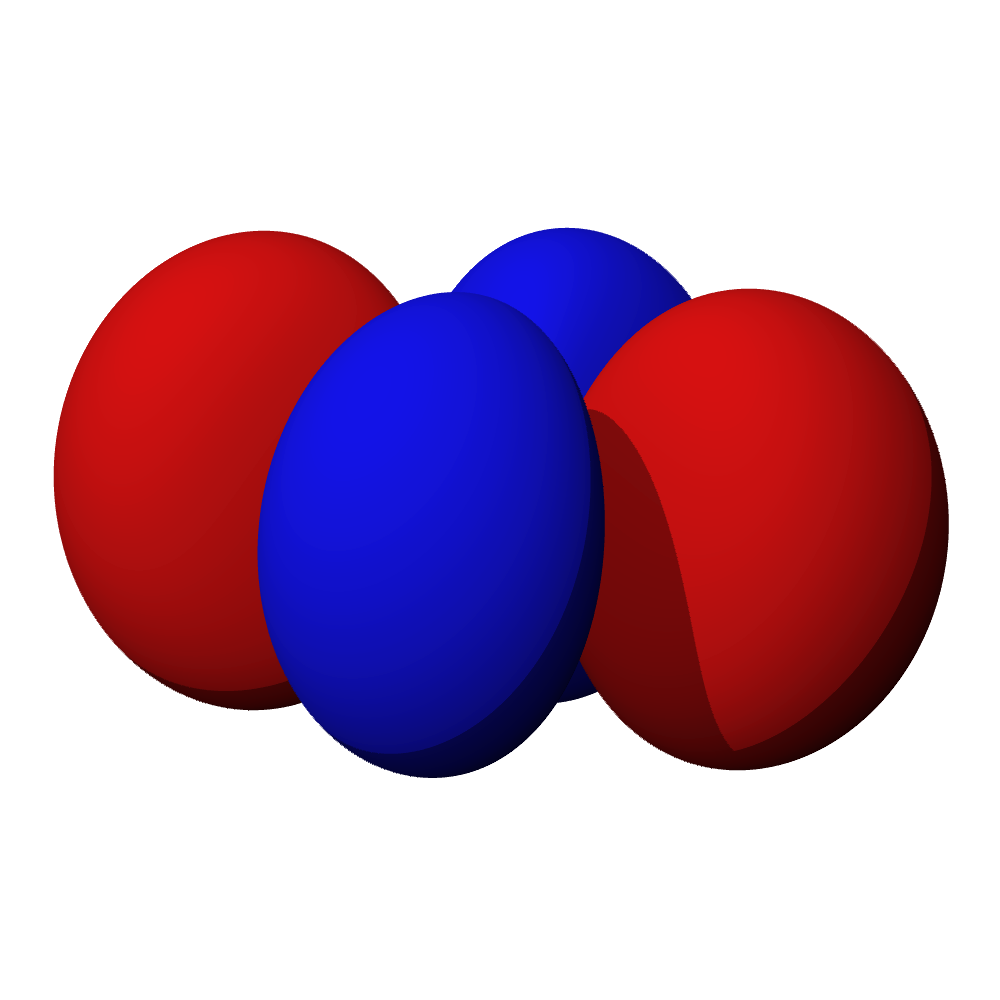
\includegraphics[width=1.6cm]{tableau_geometrie_orbitale_modelisation/Dxy_orbital.png} 
&
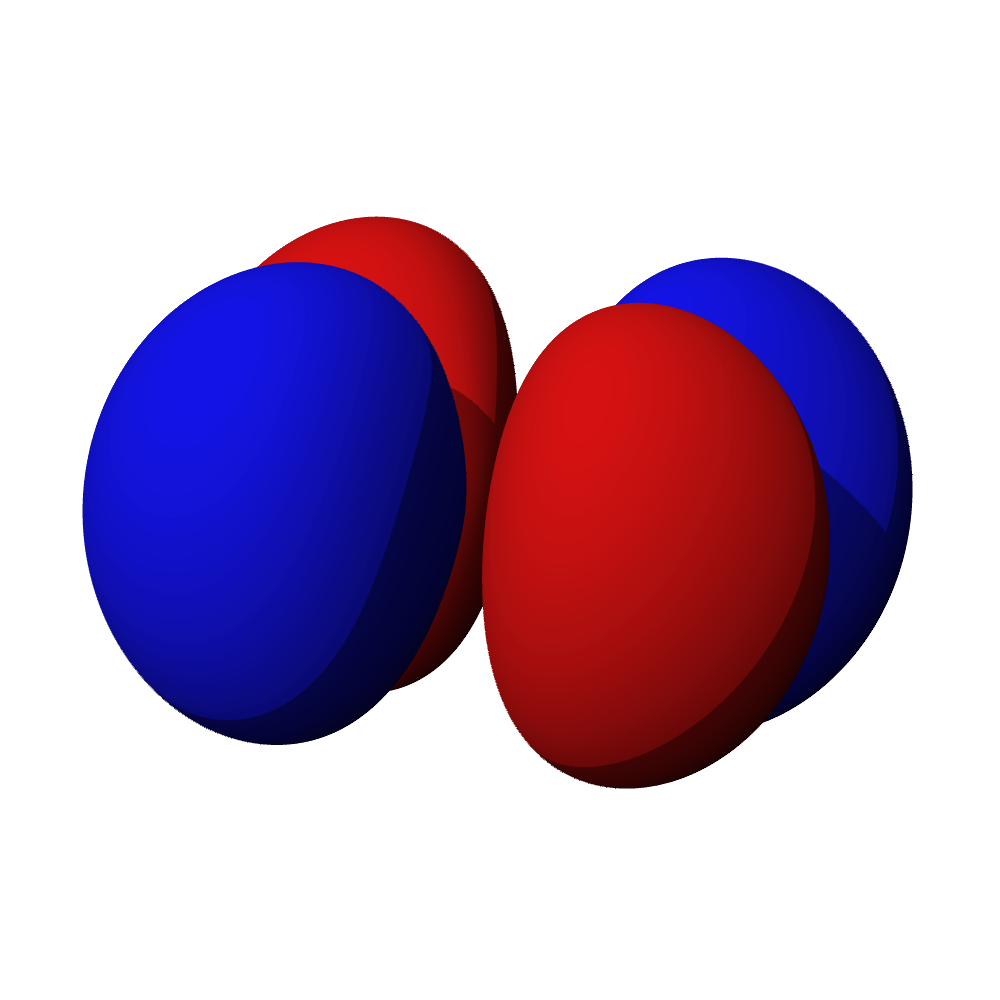
\includegraphics[width=1.6cm]{tableau_geometrie_orbitale_modelisation/Dx2-y2_orbital.png} 
& & \\
& & & \makecell[c]{$3d_{z^2}$} & \makecell[c]{$3d_{xz}$} & \makecell[c]{$3d_{yz}$} & \makecell[c]{$3d_{xy}$} & \makecell[c]{$3d_{x^{2}-y^{2}}$} & &  \\ %centrer la cellule individuellement 

\addlinespace

%\noalign{\break} %impose le saut de page au tableau tout en répartissant verticalement le tableau

\multirow[t]{8}{*}{$n=4$} & \multirow[t]{2}{*}{$\ell=0$} & \multirow[t]{2}{*}{$4s$} & 
\centering
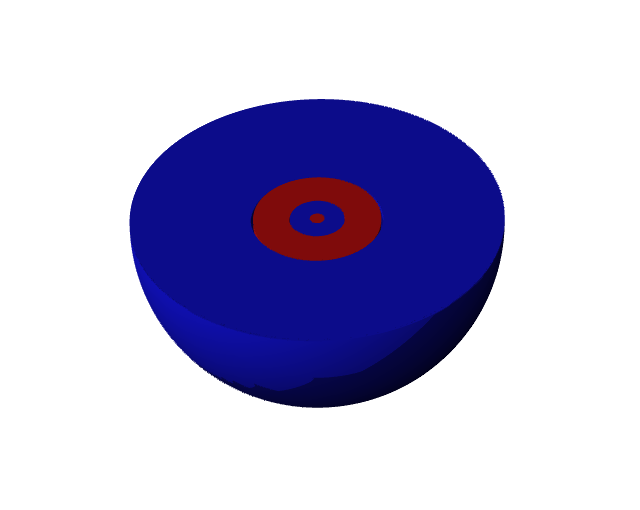
\includegraphics[width=1.6cm]{tableau_geometrie_orbitale_modelisation/S4M0.png} 
& & & & & & \\

& & & \makecell[c]{$3s$} & & & & & &  \\ %centrer la cellule individuellement 

\addlinespace

& \multirow[t]{2}{*}{$\ell=1$} & \multirow[t]{2}{*}{$4p$} & 
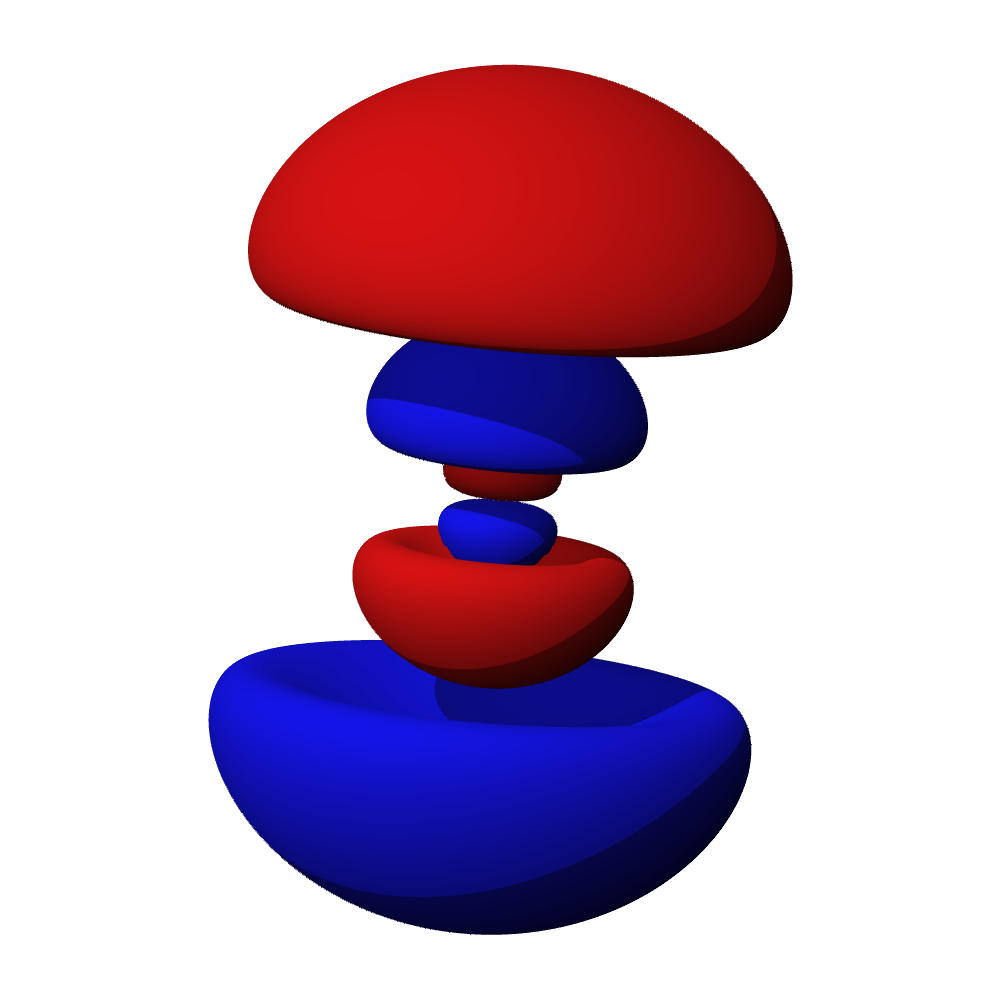
\includegraphics[width=1.6cm]{tableau_geometrie_orbitale_modelisation/P4z.png} 
&
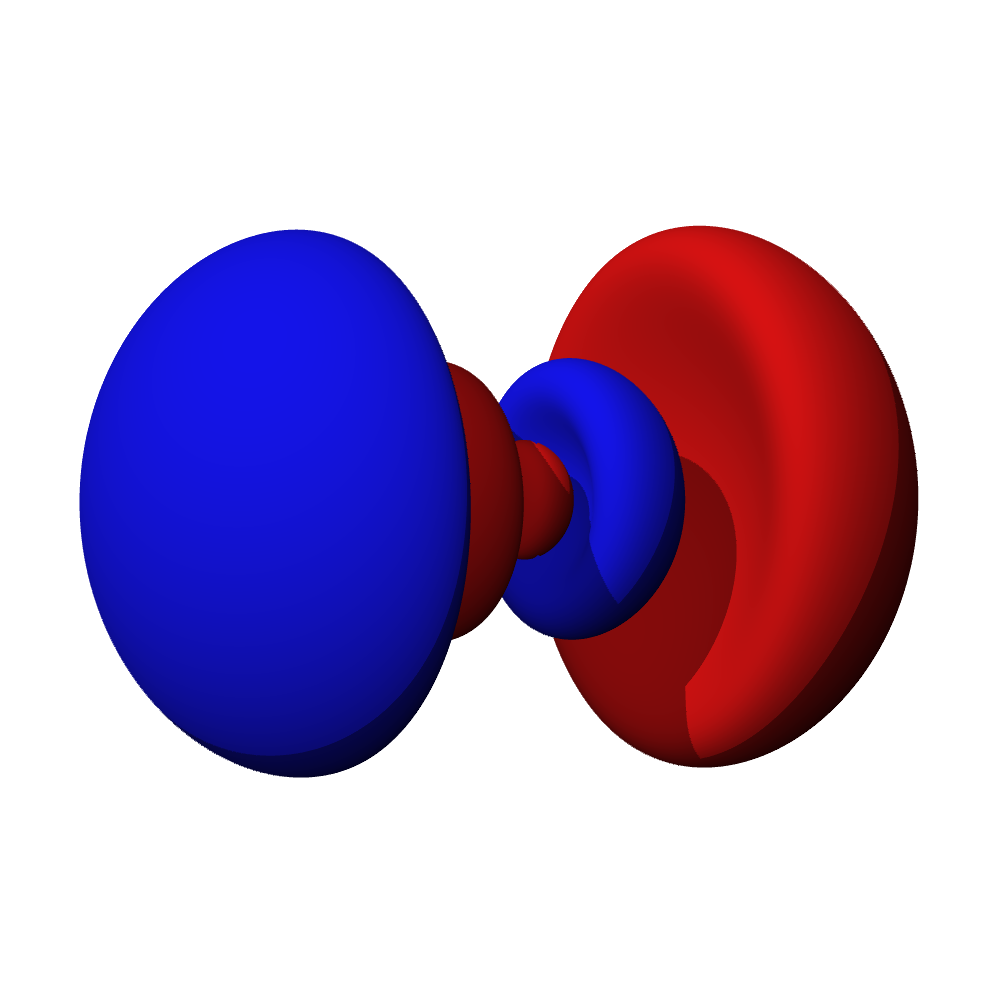
\includegraphics[width=1.6cm]{tableau_geometrie_orbitale_modelisation/P4x.png}  
&
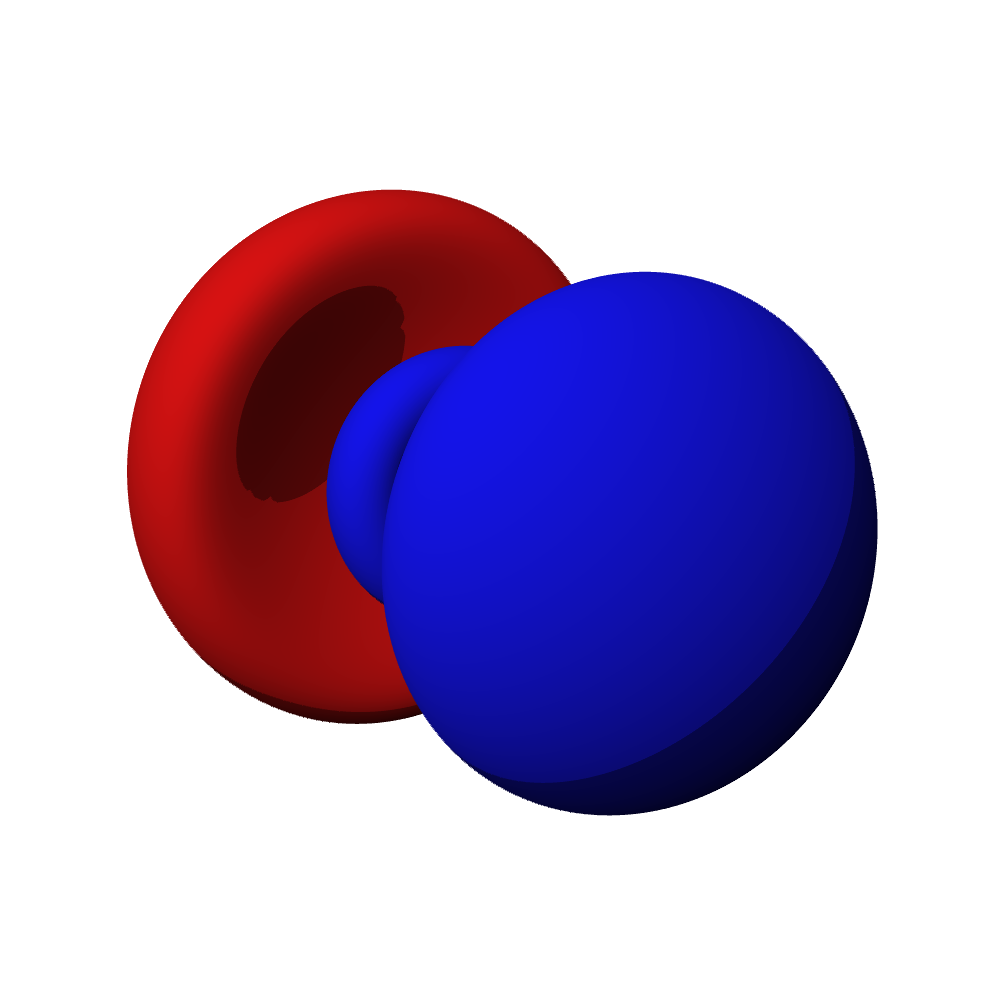
\includegraphics[width=1.6cm]{tableau_geometrie_orbitale_modelisation/P4y.png} 
& & & & \\

& & & \makecell[c]{$3p_z$} & \makecell[c]{$3p_x$} & \makecell[c]{$3p_y$} & & & &  \\ %centrer la cellule individuellement 

\addlinespace

& \multirow[t]{2}{*}{$\ell=2$} & \multirow[t]{2}{*}{$4d$} & 
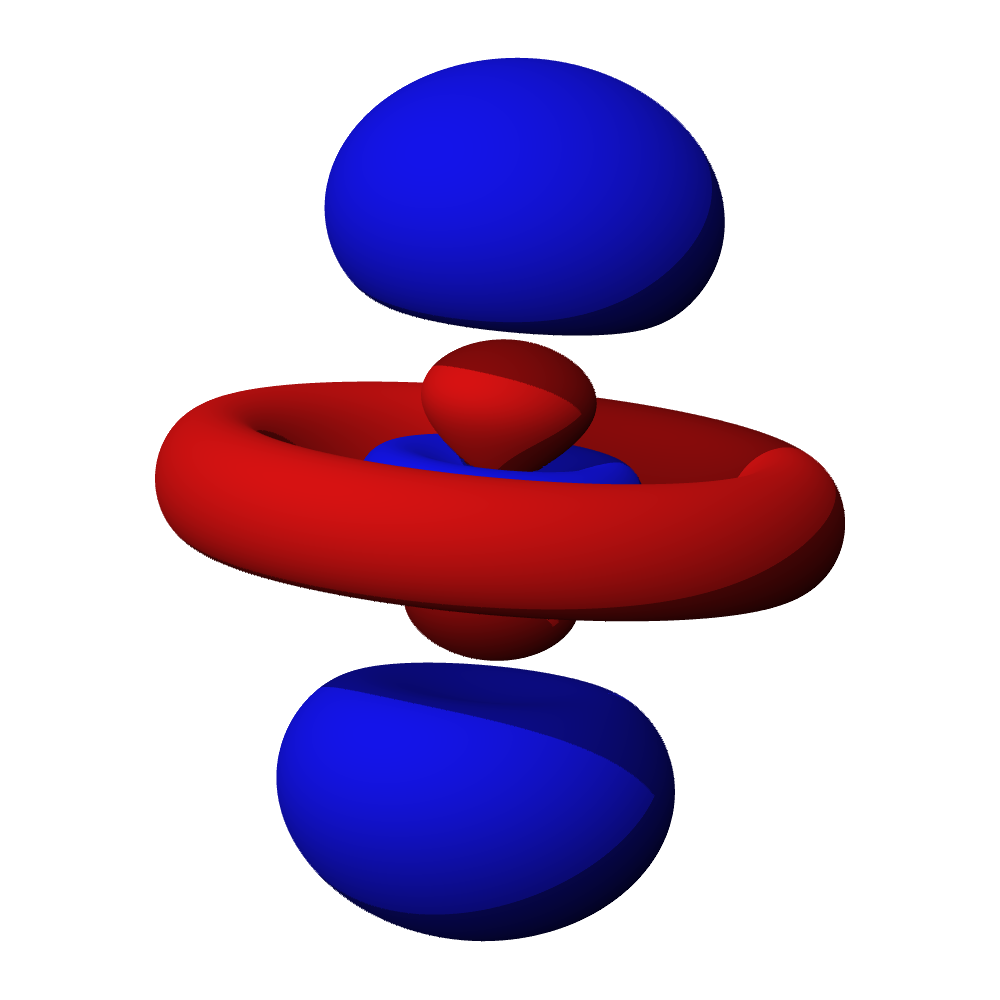
\includegraphics[width=1.6cm]{tableau_geometrie_orbitale_modelisation/D4z2.png} 
&
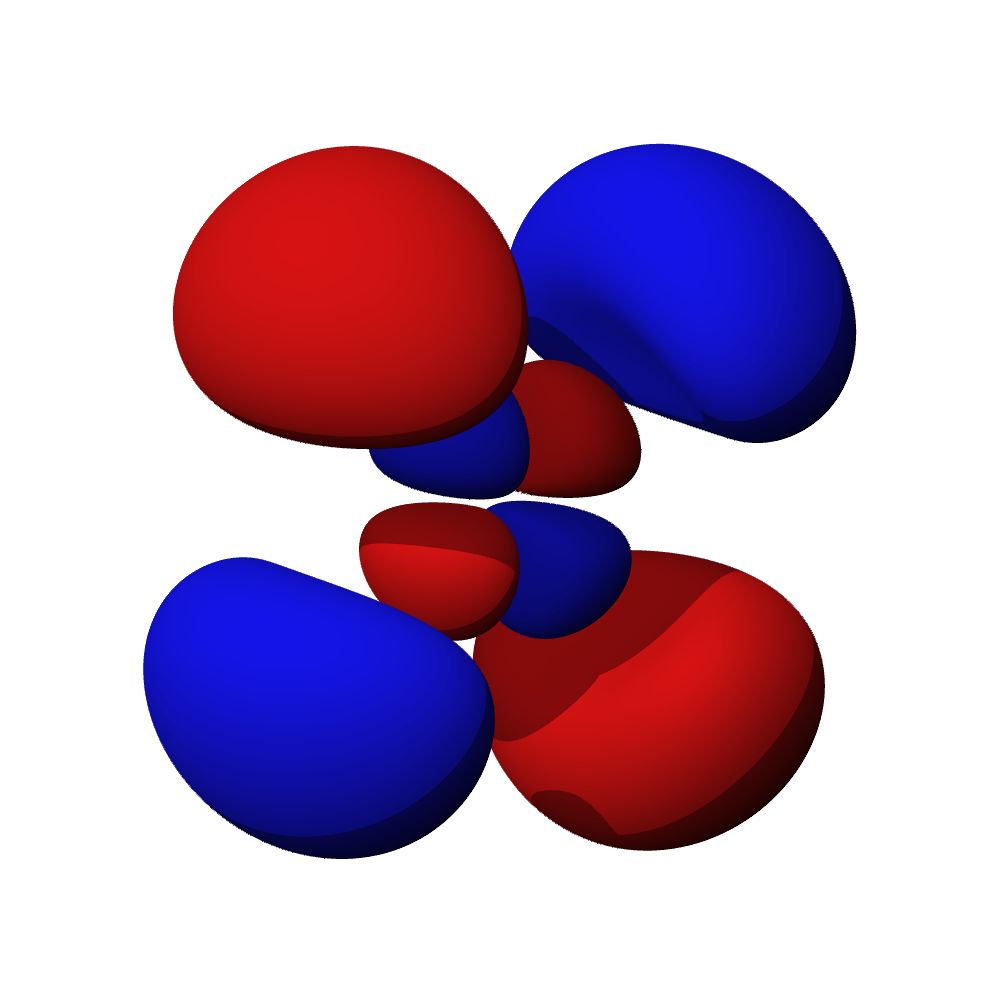
\includegraphics[width=1.6cm]{tableau_geometrie_orbitale_modelisation/D4xz.png}  
&
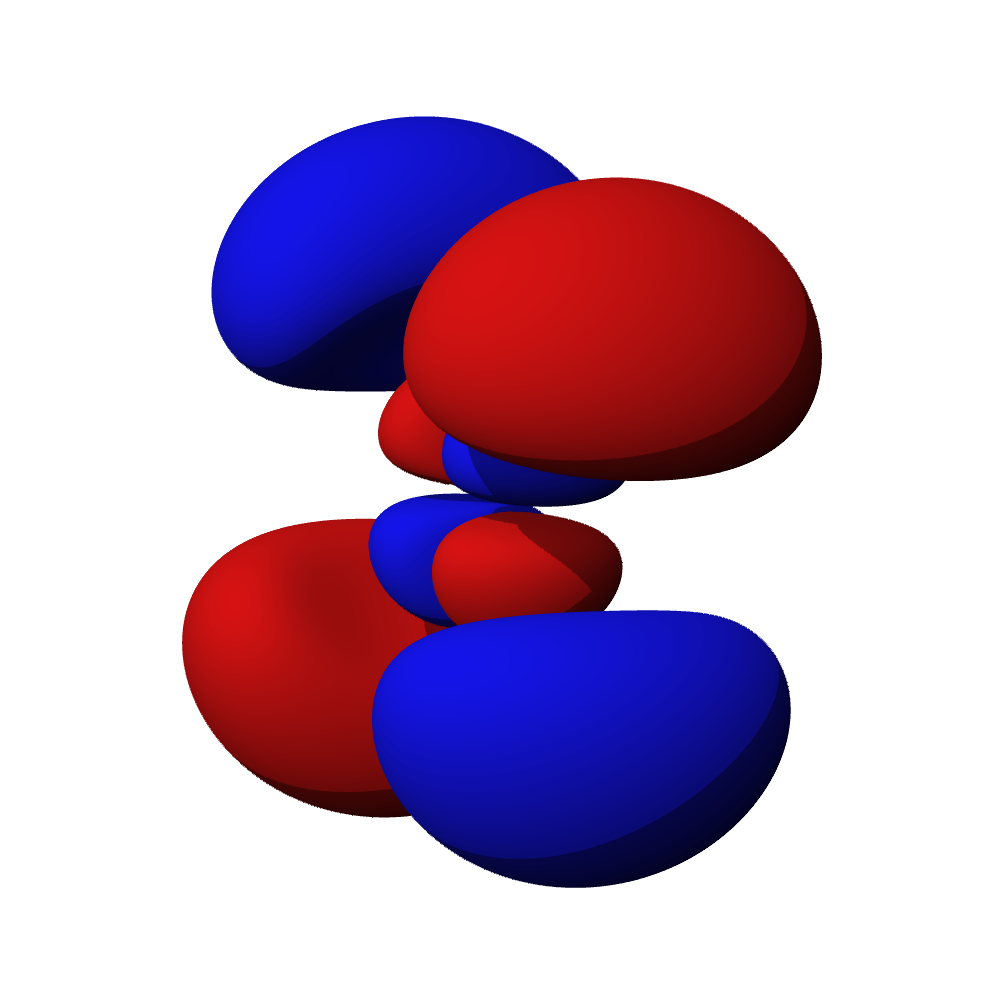
\includegraphics[width=1.6cm]{tableau_geometrie_orbitale_modelisation/D4yz.png} 
& 
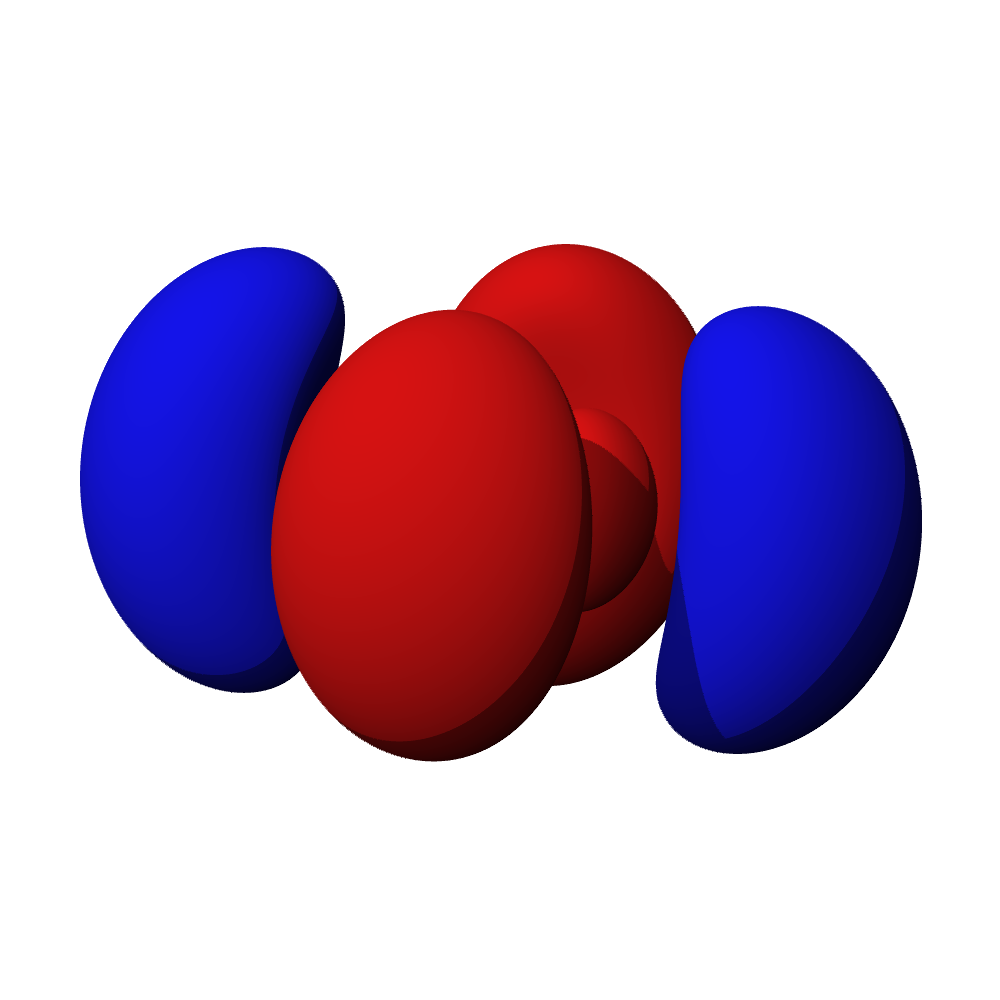
\includegraphics[width=1.6cm]{tableau_geometrie_orbitale_modelisation/D4xy.png} 
&
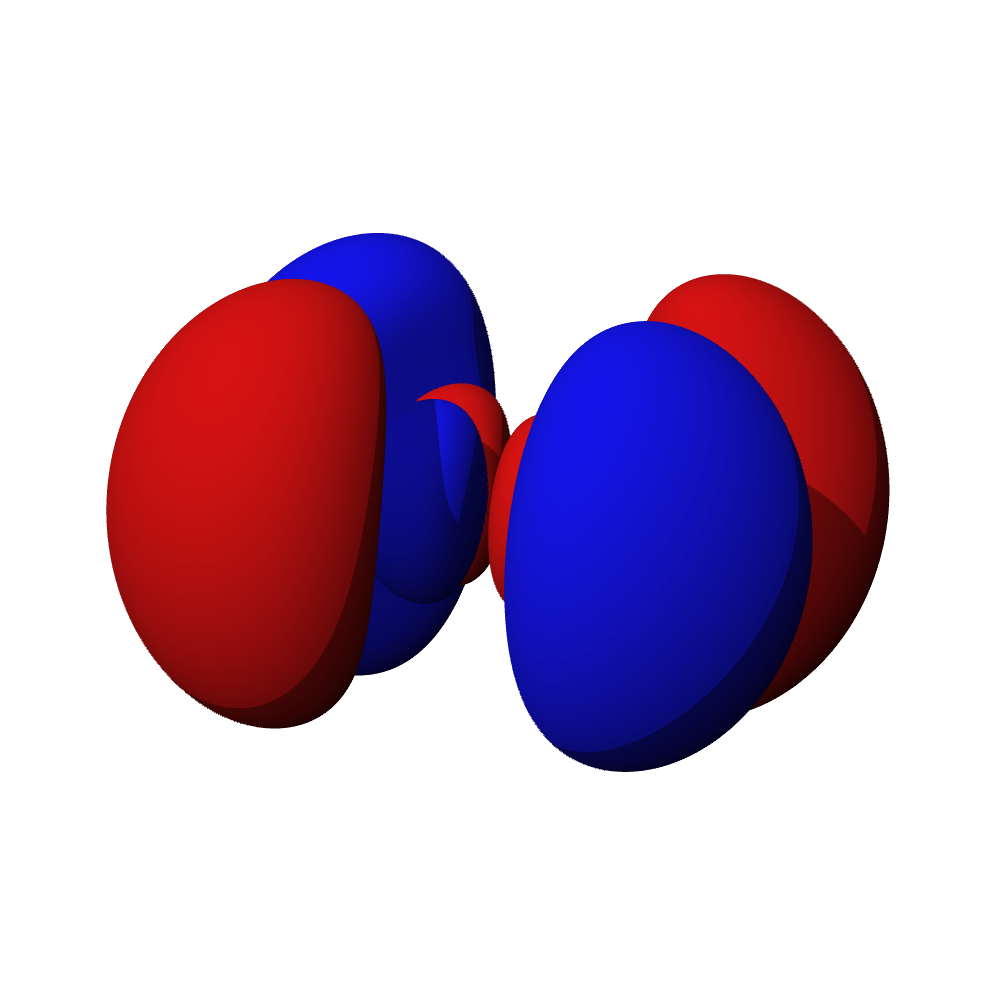
\includegraphics[width=1.6cm]{tableau_geometrie_orbitale_modelisation/D4x2-y2.png} 
& & \\

& & & \makecell[c]{$3d_{z^2}$} & \makecell[c]{$3d_{xz}$} & \makecell[c]{$3d_{yz}$} & \makecell[c]{$3d_{xy}$} & \makecell[c]{$3d_{x^{2}-y^{2}}$} & &  \\ %centrer la cellule individuellement 

\addlinespace

& \multirow[t]{2}{*}{$\ell=3$} & \multirow[t]{2}{*}{$4f$} & 
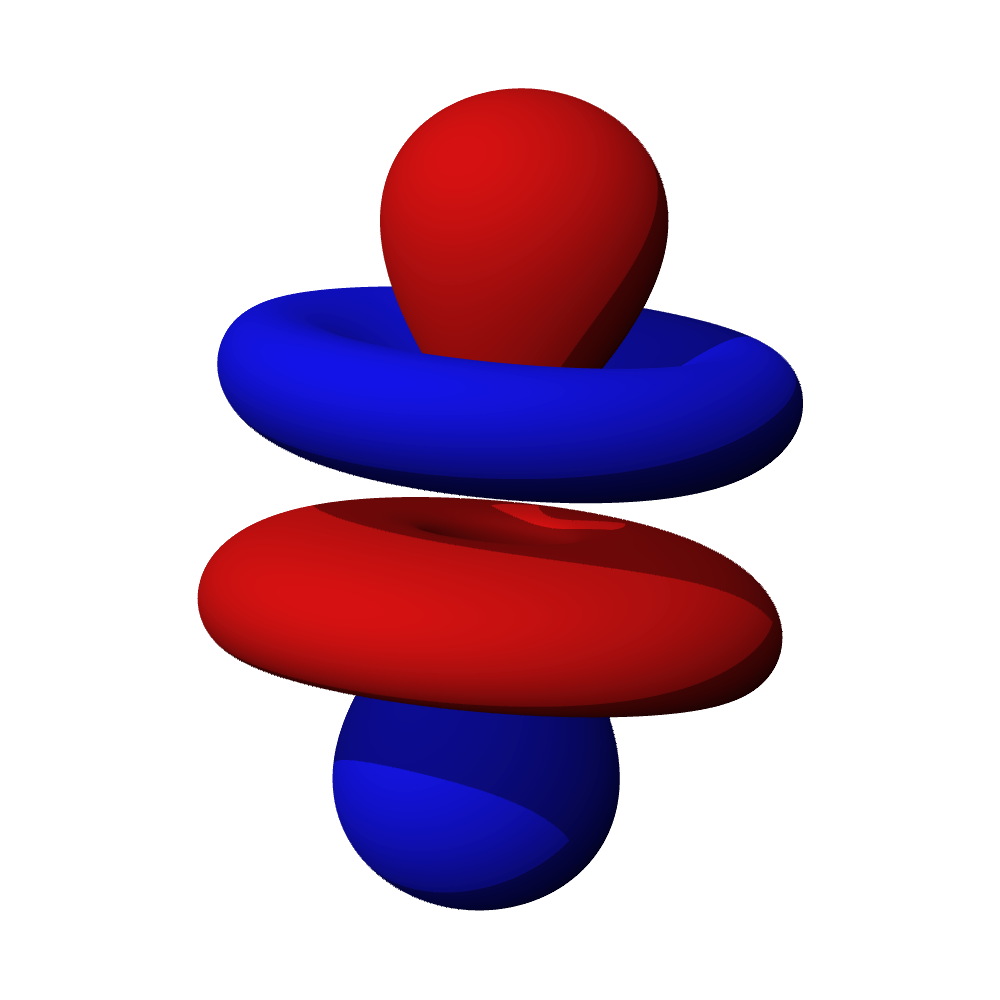
\includegraphics[width=1.6cm]{tableau_geometrie_orbitale_modelisation/Fz3_orbital.png} 
&
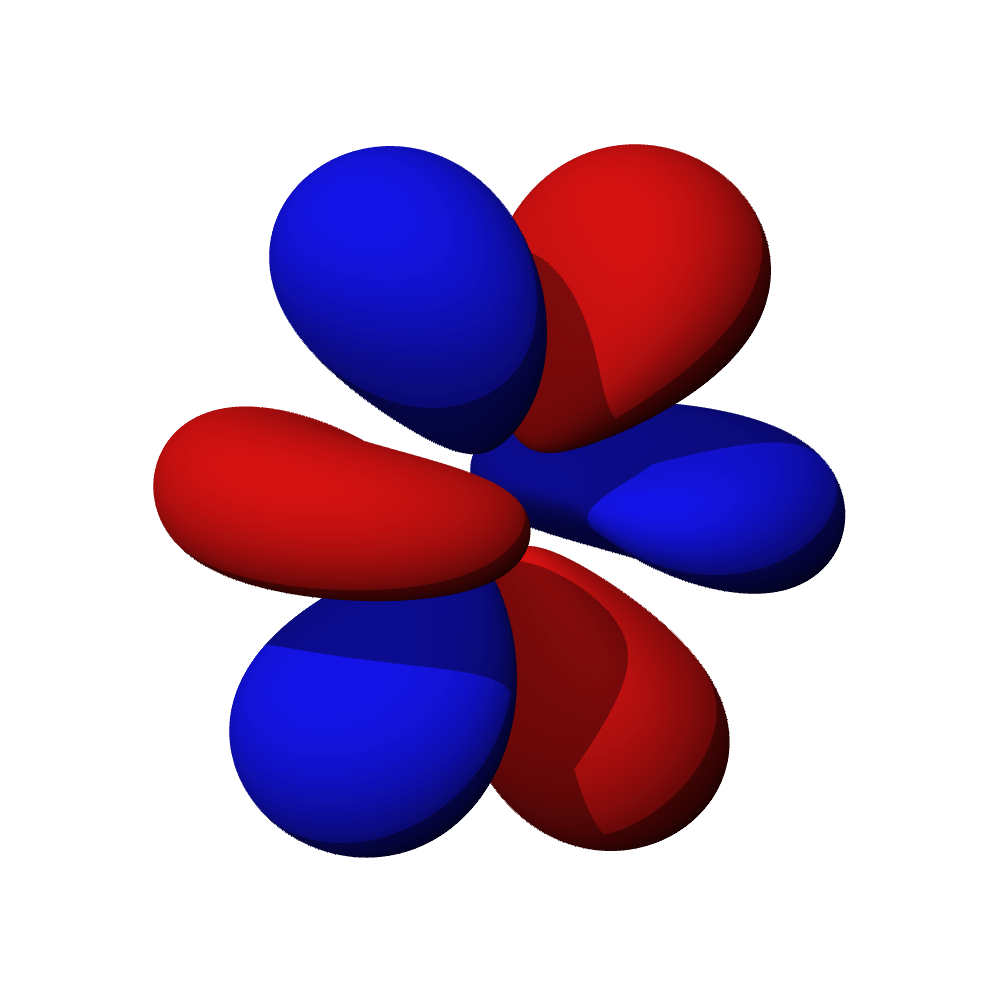
\includegraphics[width=1.6cm]{tableau_geometrie_orbitale_modelisation/Fxz2_orbital.png}  
&
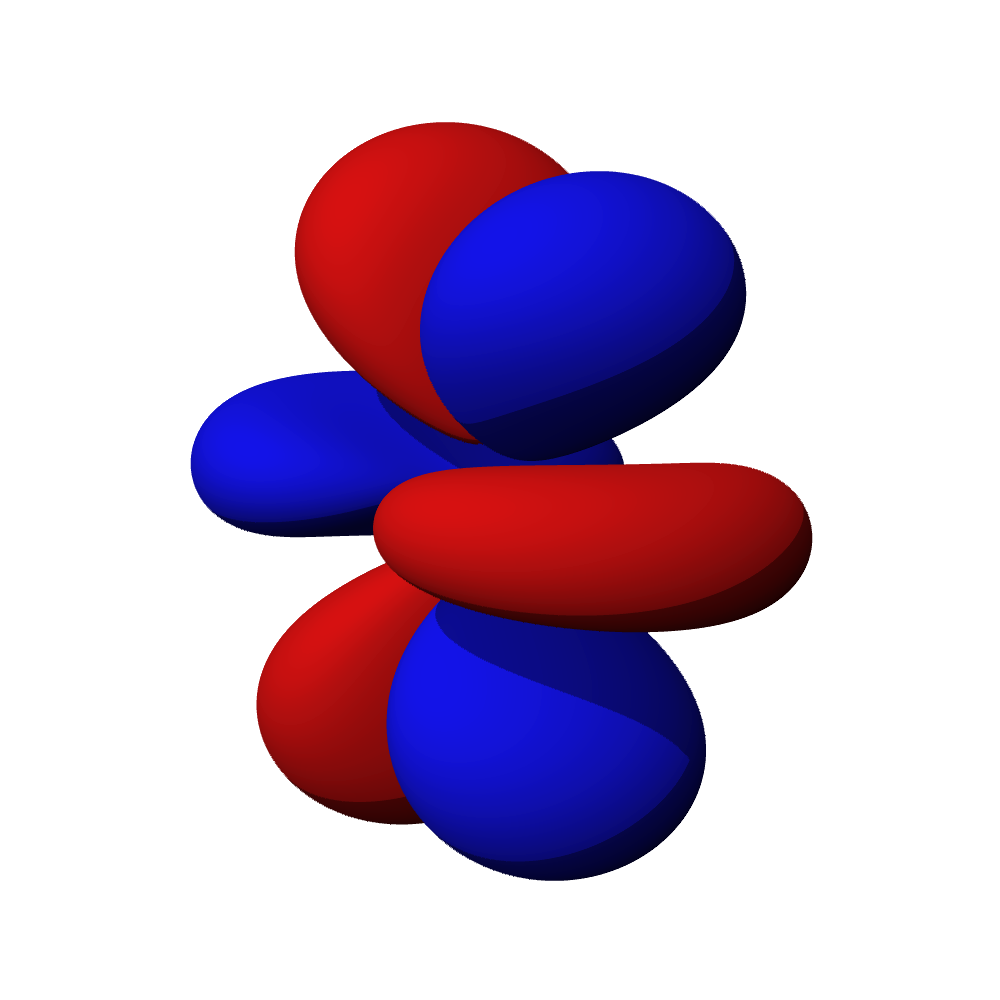
\includegraphics[width=1.6cm]{tableau_geometrie_orbitale_modelisation/Fyz2_orbital.png} 
& 
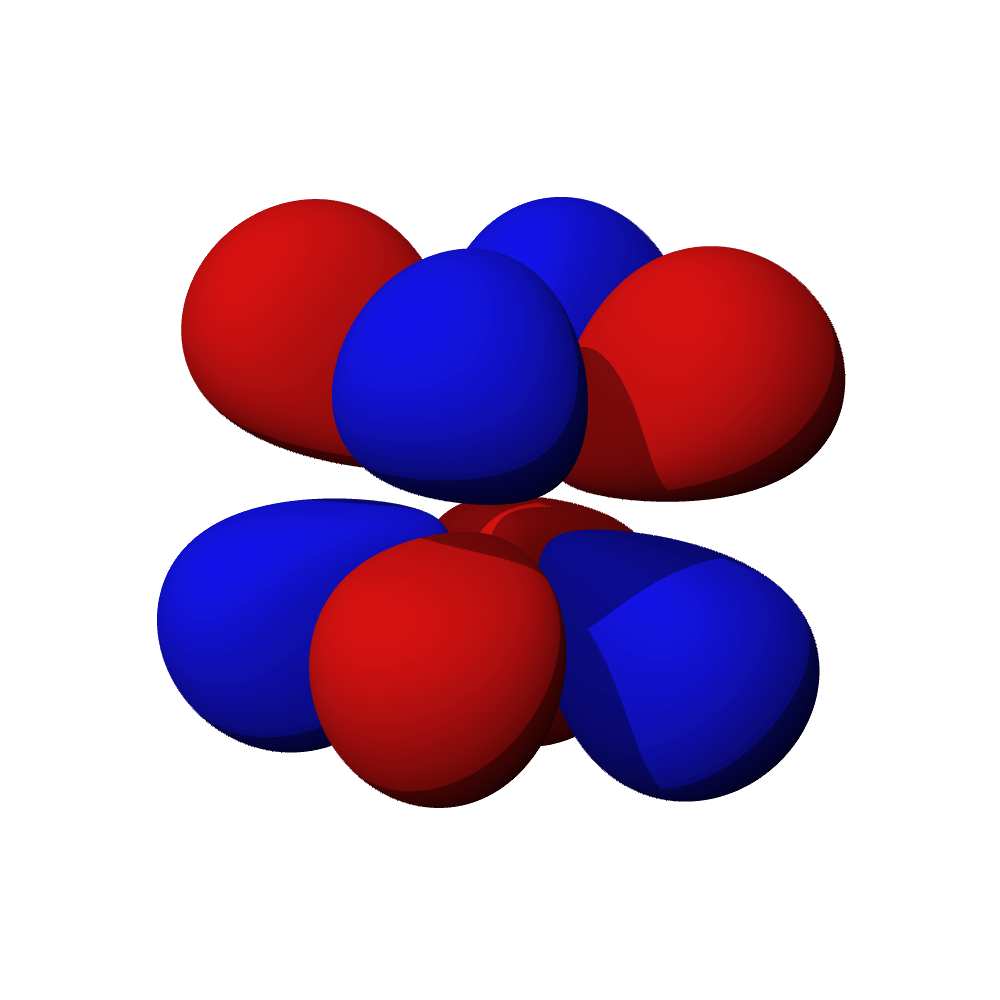
\includegraphics[width=1.6cm]{tableau_geometrie_orbitale_modelisation/Fxyz_orbital.png} 
&
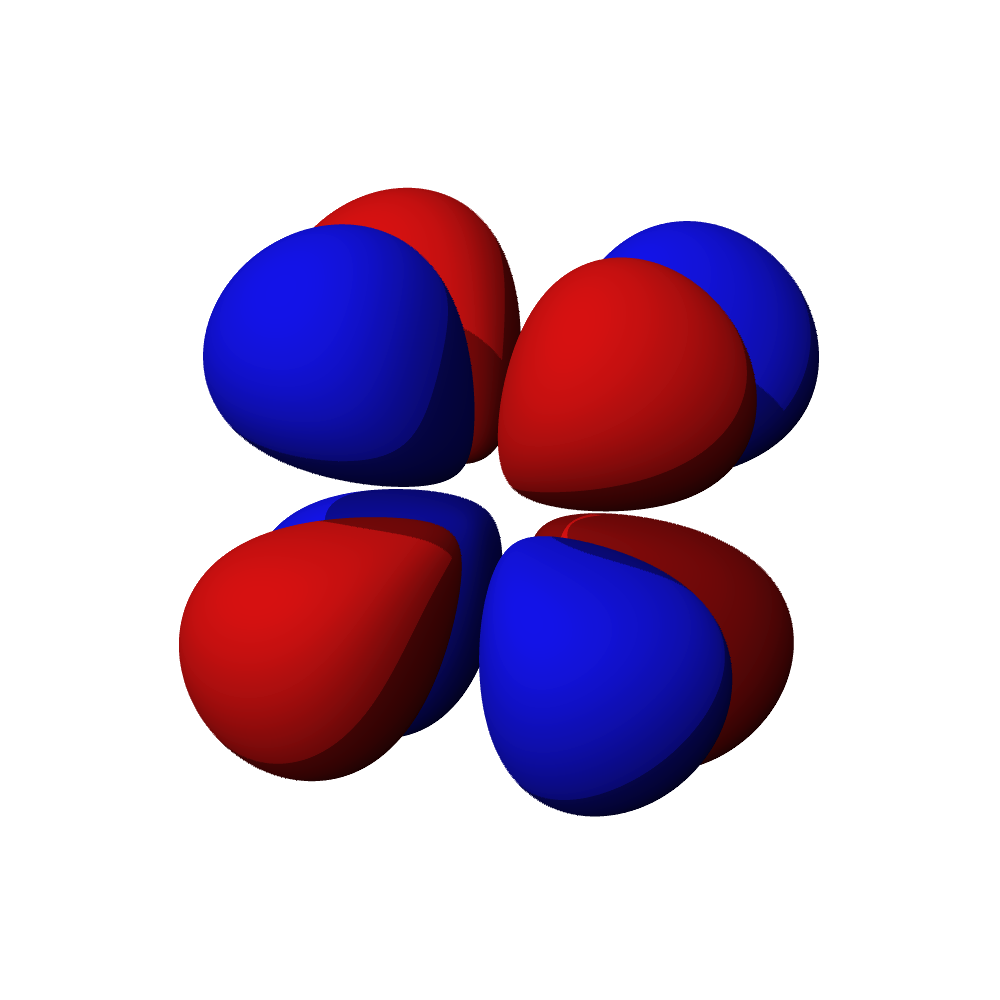
\includegraphics[width=1.6cm]{tableau_geometrie_orbitale_modelisation/Fz(x2-y2)_orbital.png} 
& 
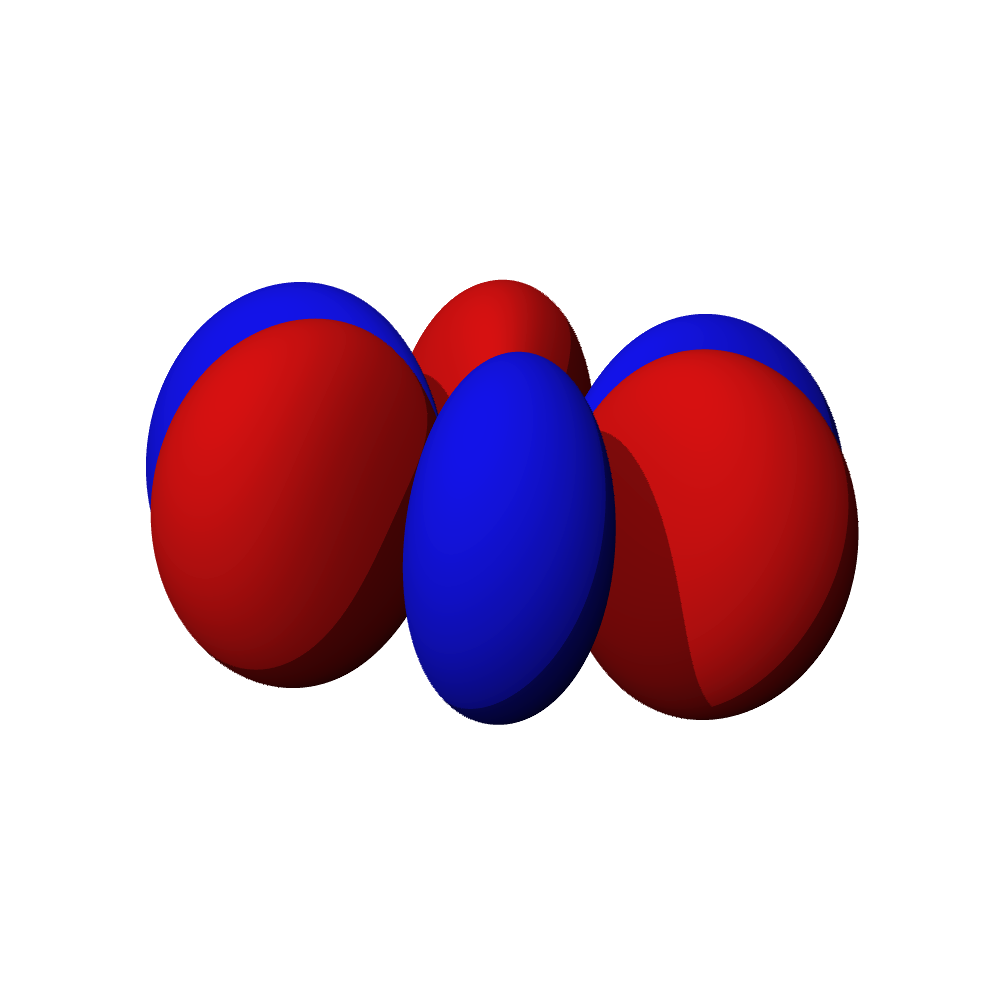
\includegraphics[width=1.6cm]{tableau_geometrie_orbitale_modelisation/Fx(x2-3y2)_orbital.png}
&
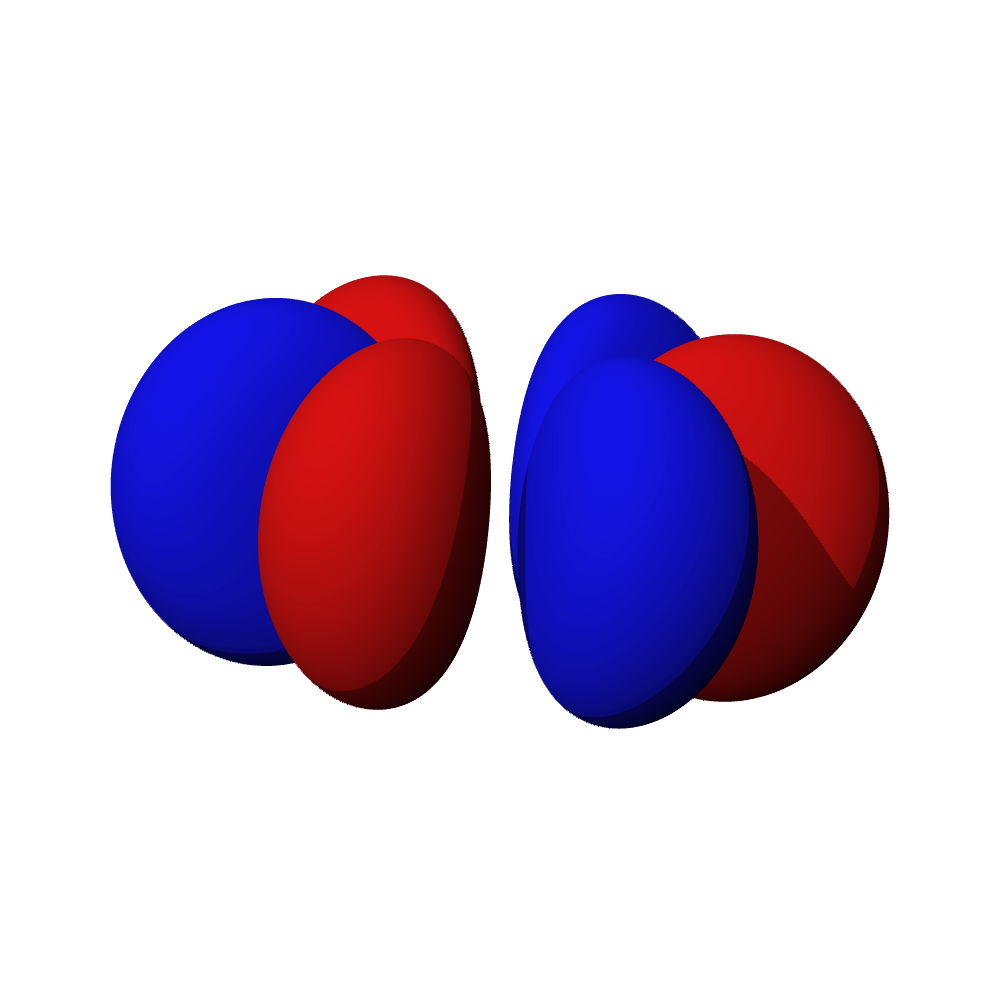
\includegraphics[width=1.6cm]{tableau_geometrie_orbitale_modelisation/Fy(3x2-y2)_orbital.png} \\

& & & \makecell[c]{$4f_{z^3}$} & \makecell[c]{$4f_{xz^2}$} & \makecell[c]{$4f_{yz^2}$} & \makecell[c]%
{$4f_{xyz}$} & \makecell[c]{$4f_{z(x^{2}-y^2)}$} & \makecell[c]{$4f_{x(x^{2}-y^2)}$} & \makecell[c]%
{$4f_{y(x^{2}-y^2)}$} \\ %centrer la cellule individuellement 

\midrule %filet de milieu de tableau

\multirow[t]{4}{*}{$n=5$} & \multirow[t]{2}{*}{$\ell=0$} & \multirow[t]{2}{*}{$5s$} & 
\centering
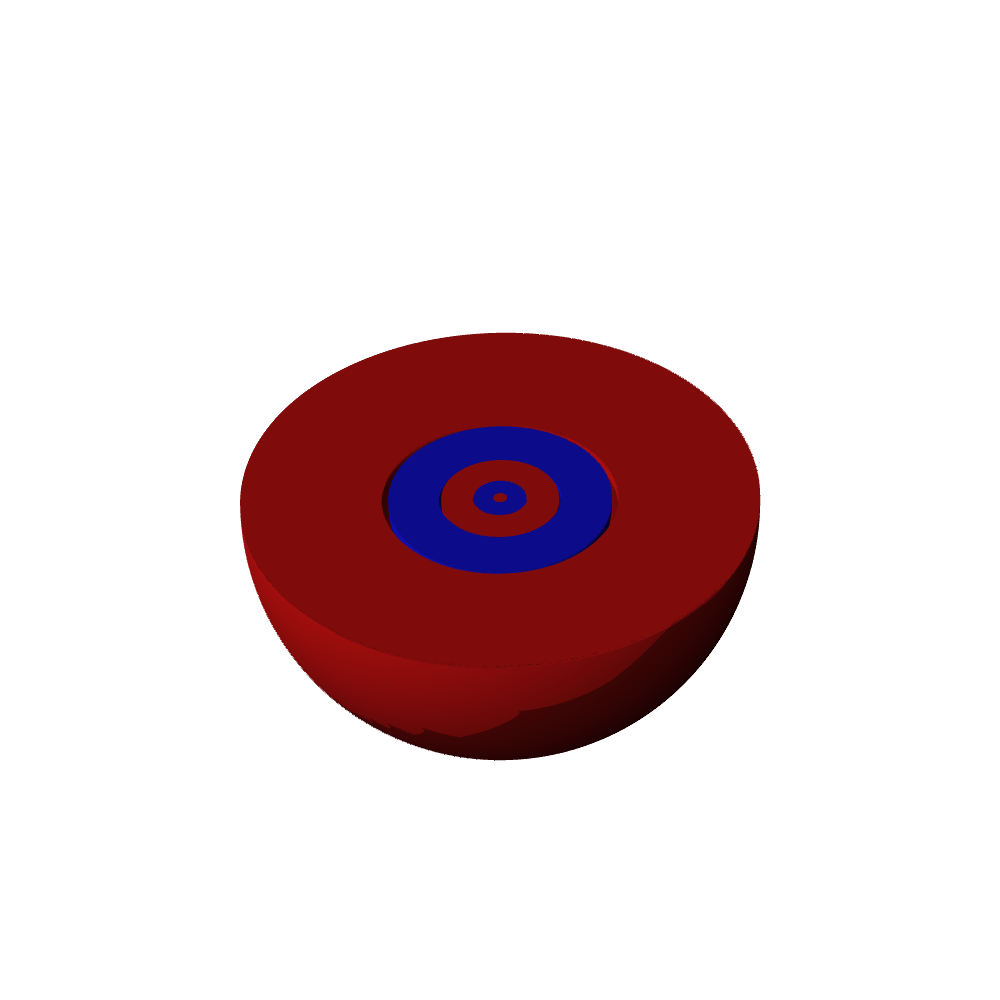
\includegraphics[width=1.6cm]{tableau_geometrie_orbitale_modelisation/S5M0.png} 
& & & & & & \\

& & & \makecell[c]{$5s$} & & & & & &  \\ %centrer la cellule individuellement 

\addlinespace

& \multirow[t]{2}{*}{$\ell=1$} & \multirow[t]{2}{*}{$5p$} & 
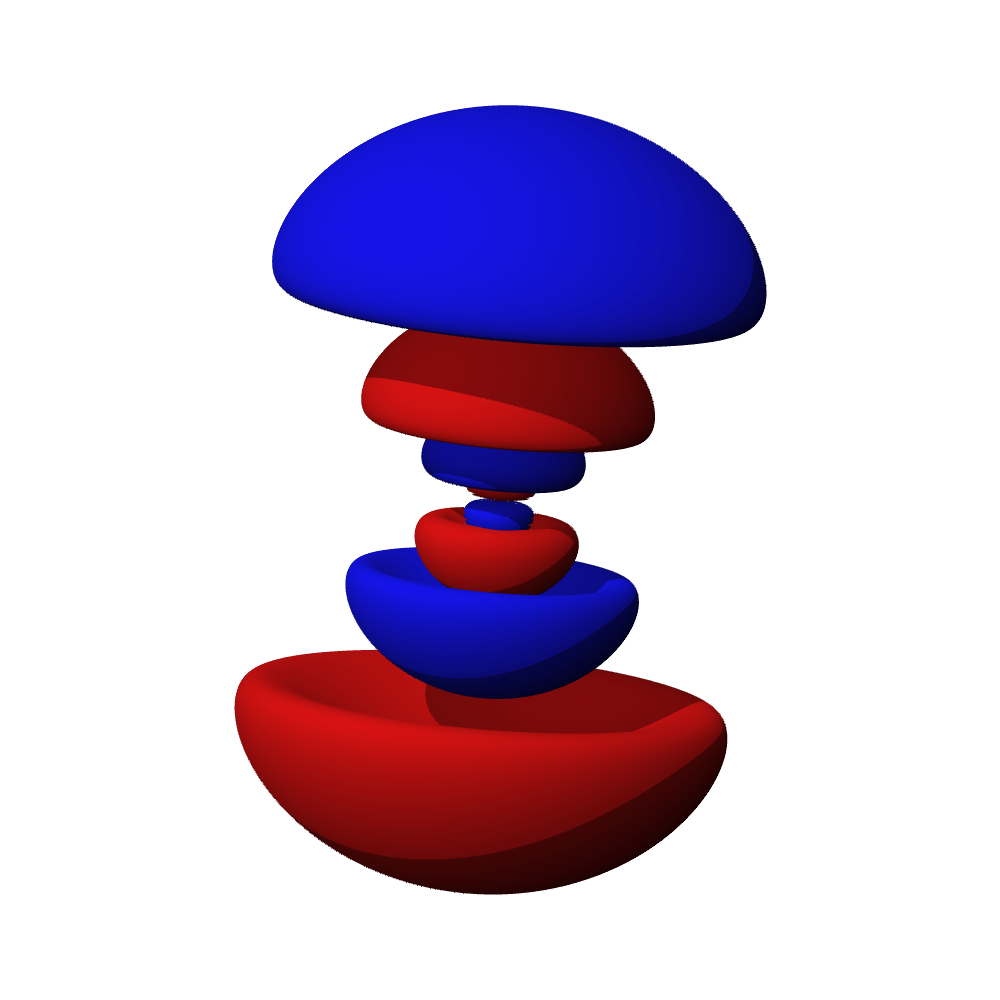
\includegraphics[width=1.6cm]{tableau_geometrie_orbitale_modelisation/P5z.png} 
&
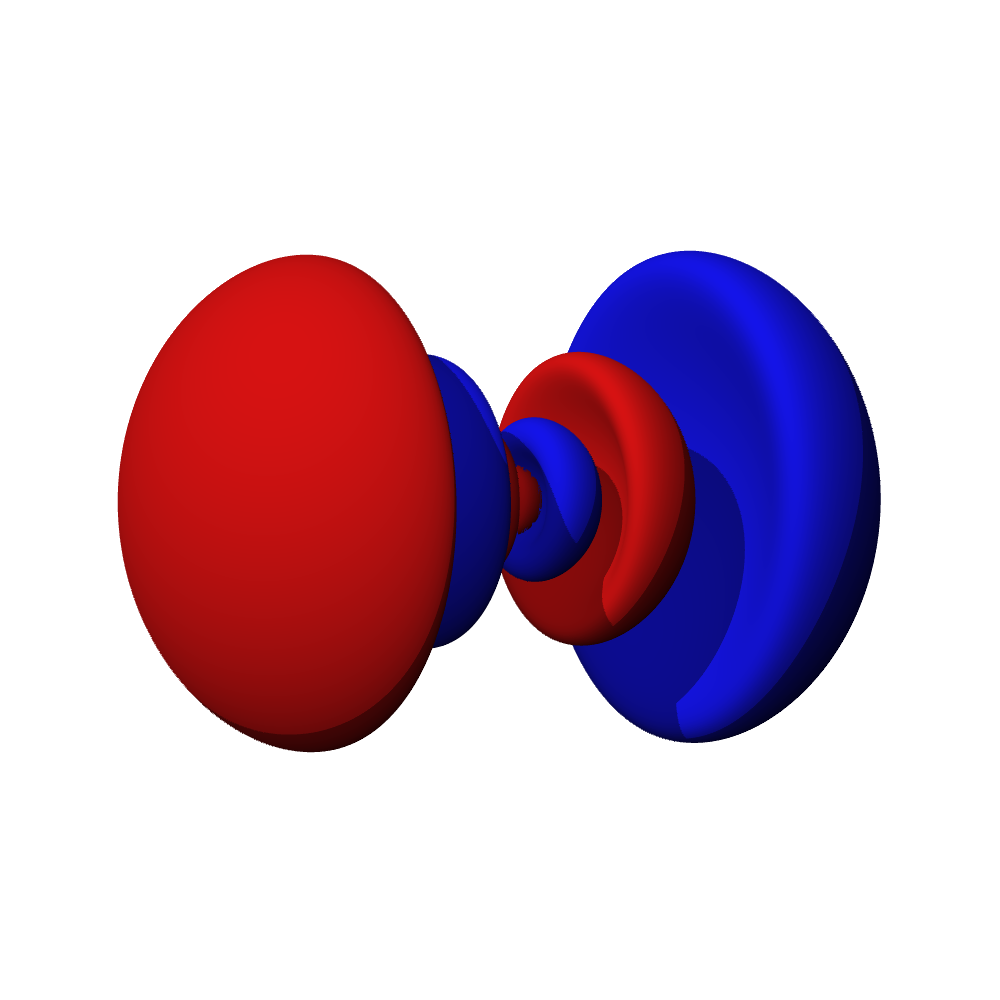
\includegraphics[width=1.6cm]{tableau_geometrie_orbitale_modelisation/P5x.png}  
&
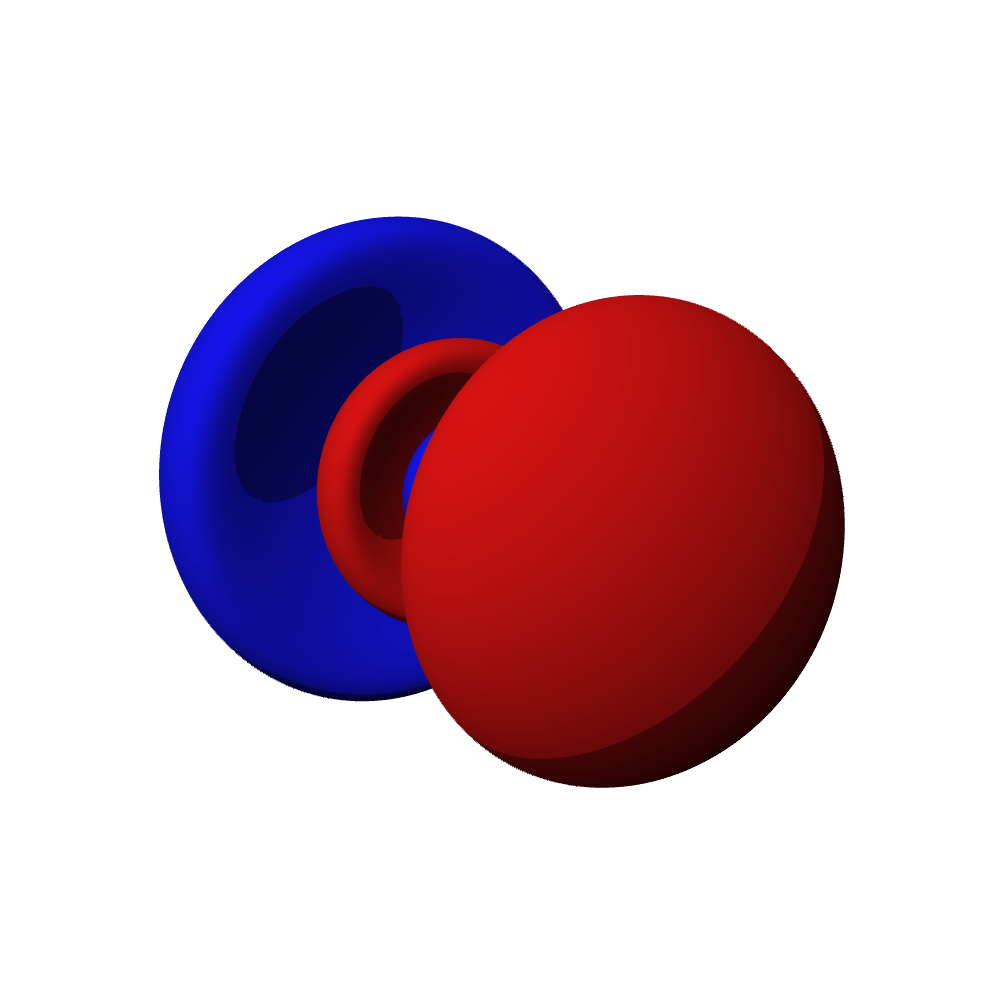
\includegraphics[width=1.6cm]{tableau_geometrie_orbitale_modelisation/P5y.png} 
& & & & \\

& & & \makecell[c]{$5p_z$} & \makecell[c]{$5p_x$} & \makecell[c]{$5p_y$} & & & &  \\ %centrer la cellule individuellement 

\addlinespace

\multirow[t]{2}{*}{$n=5$} & \multirow[t]{2}{*}{$\ell=2$} & \multirow[t]{2}{*}{$5d$} & 
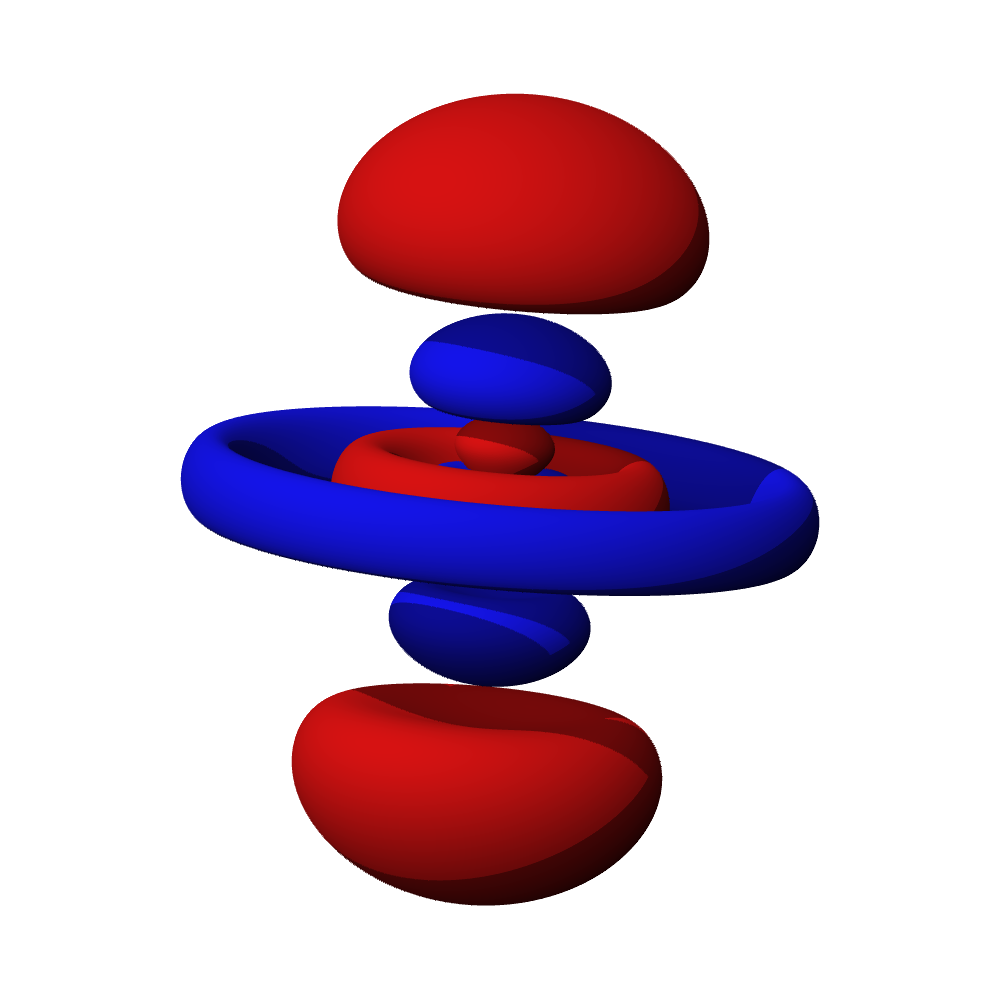
\includegraphics[width=1.6cm]{tableau_geometrie_orbitale_modelisation/D5z2.png} 
&
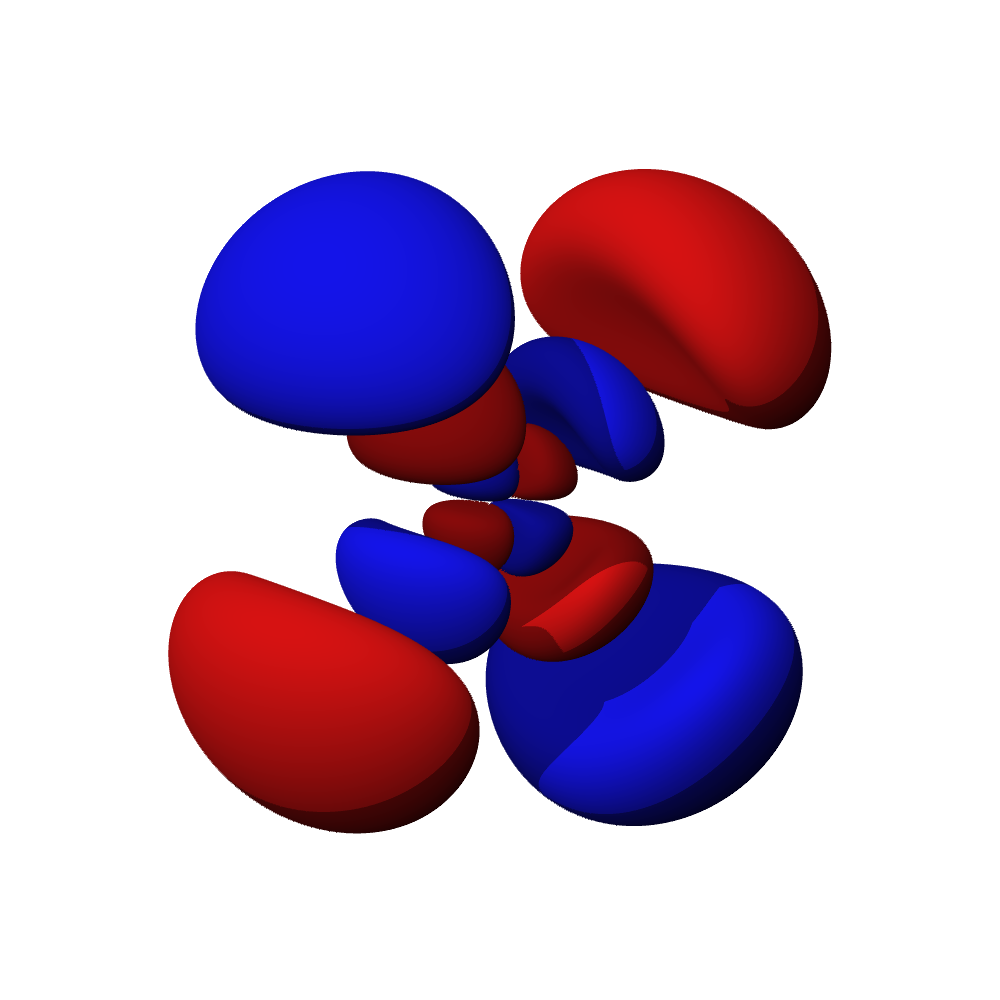
\includegraphics[width=1.6cm]{tableau_geometrie_orbitale_modelisation/D5xz.png}  
&
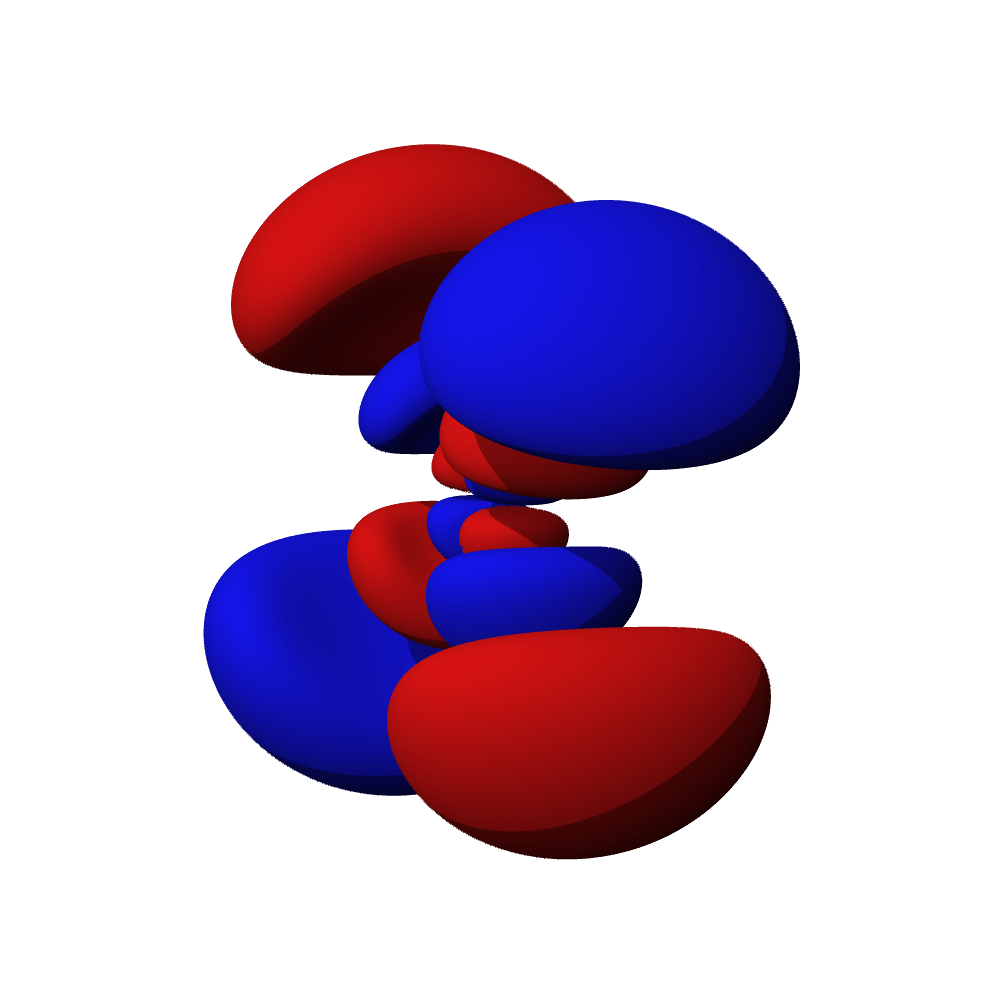
\includegraphics[width=1.6cm]{tableau_geometrie_orbitale_modelisation/D5yz.png} 
& 
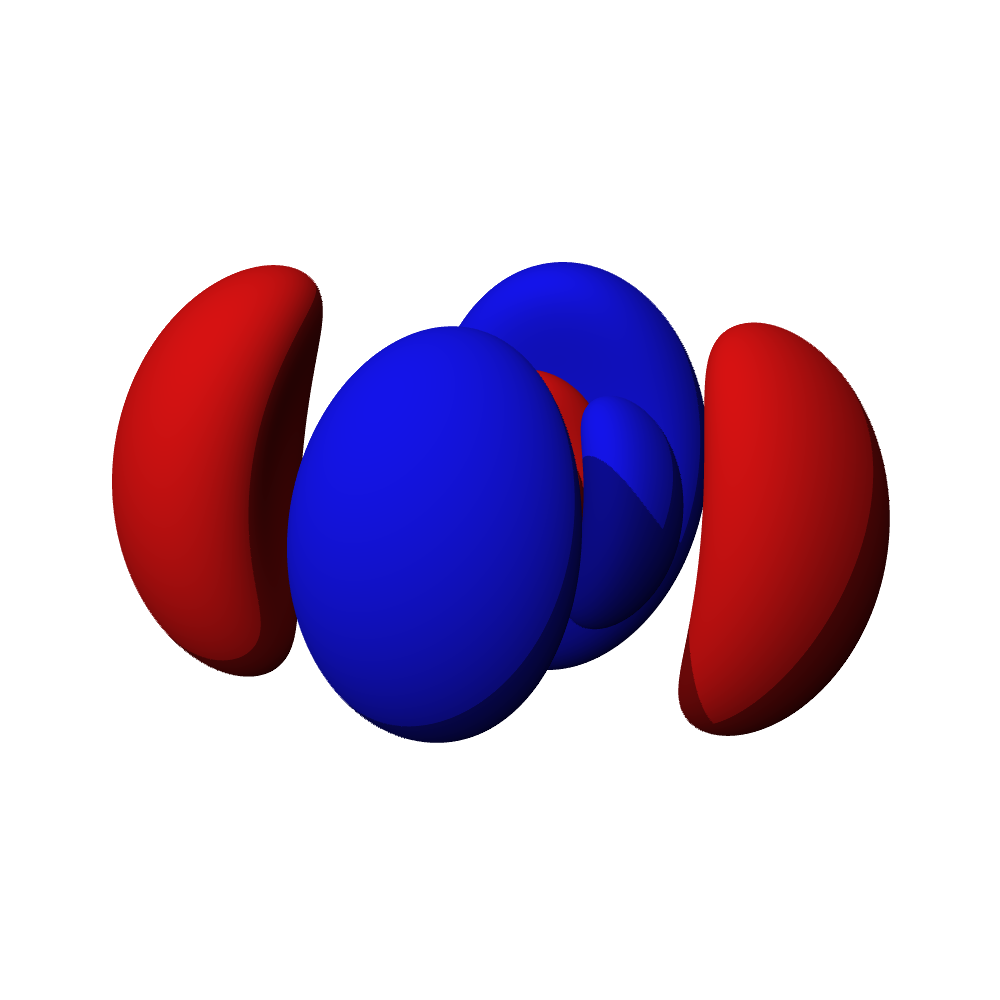
\includegraphics[width=1.6cm]{tableau_geometrie_orbitale_modelisation/D5xy.png} 
&
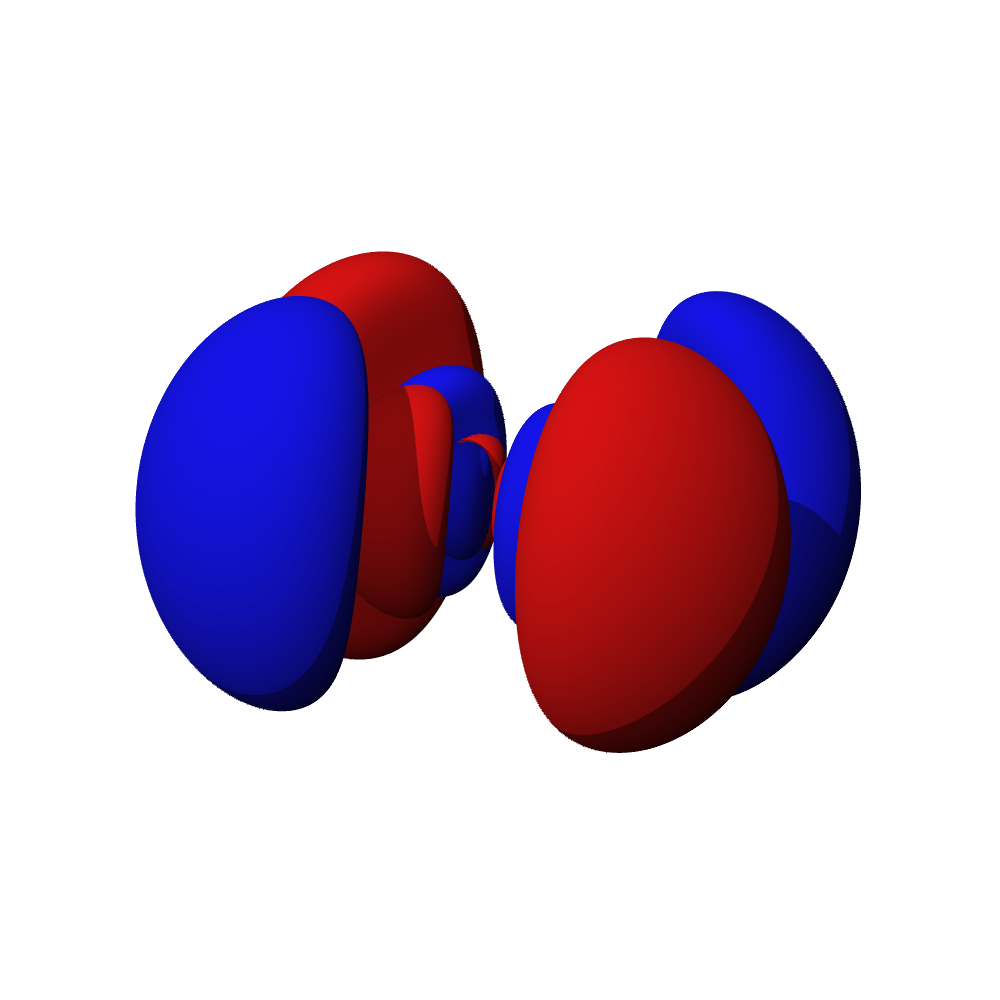
\includegraphics[width=1.6cm]{tableau_geometrie_orbitale_modelisation/D5x2-y2.png} 
& & \\
& & & \makecell[c]{$5d_{z^2}$} & \makecell[c]{$5d_{xz}$} & \makecell[c]{$5d_{yz}$} & \makecell[c]{$5d_{xy}$} & \makecell[c]{$5d_{x^{2}-y^{2}}$} & &  \\ %centrer la cellule individuellement 

\midrule

\multirow[t]{6}{*}{$n=6$} & \multirow[t]{2}{*}{$\ell=0$} & \multirow[t]{2}{*}{$6s$} & 
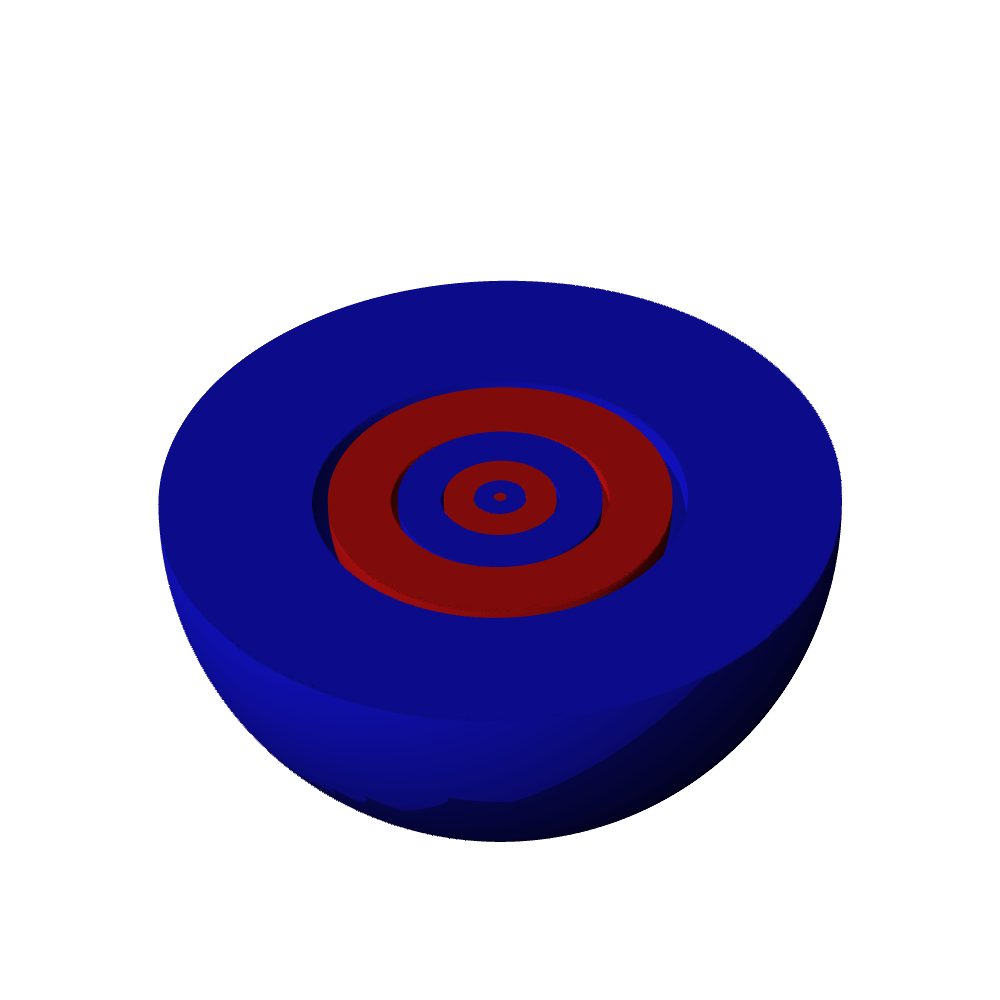
\includegraphics[width=1.6cm]{tableau_geometrie_orbitale_modelisation/S6M0.png} 
& & & & & & \\

& & & \makecell[c]{$6s$} & & & & & &  \\ %centrer la cellule individuellement 

\addlinespace

& \multirow[t]{2}{*}{$\ell=1$} & \multirow[t]{2}{*}{$6p$} & 
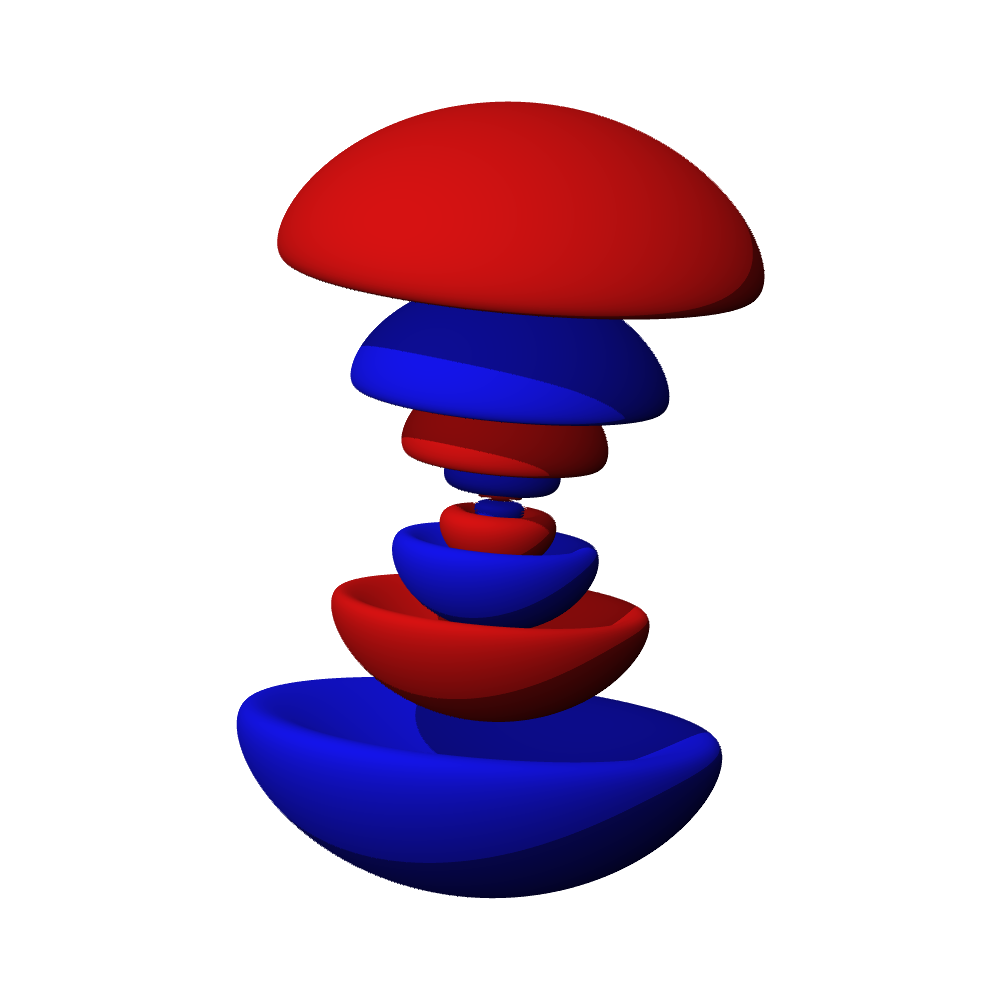
\includegraphics[width=1.6cm]{tableau_geometrie_orbitale_modelisation/P6z.png} 
&
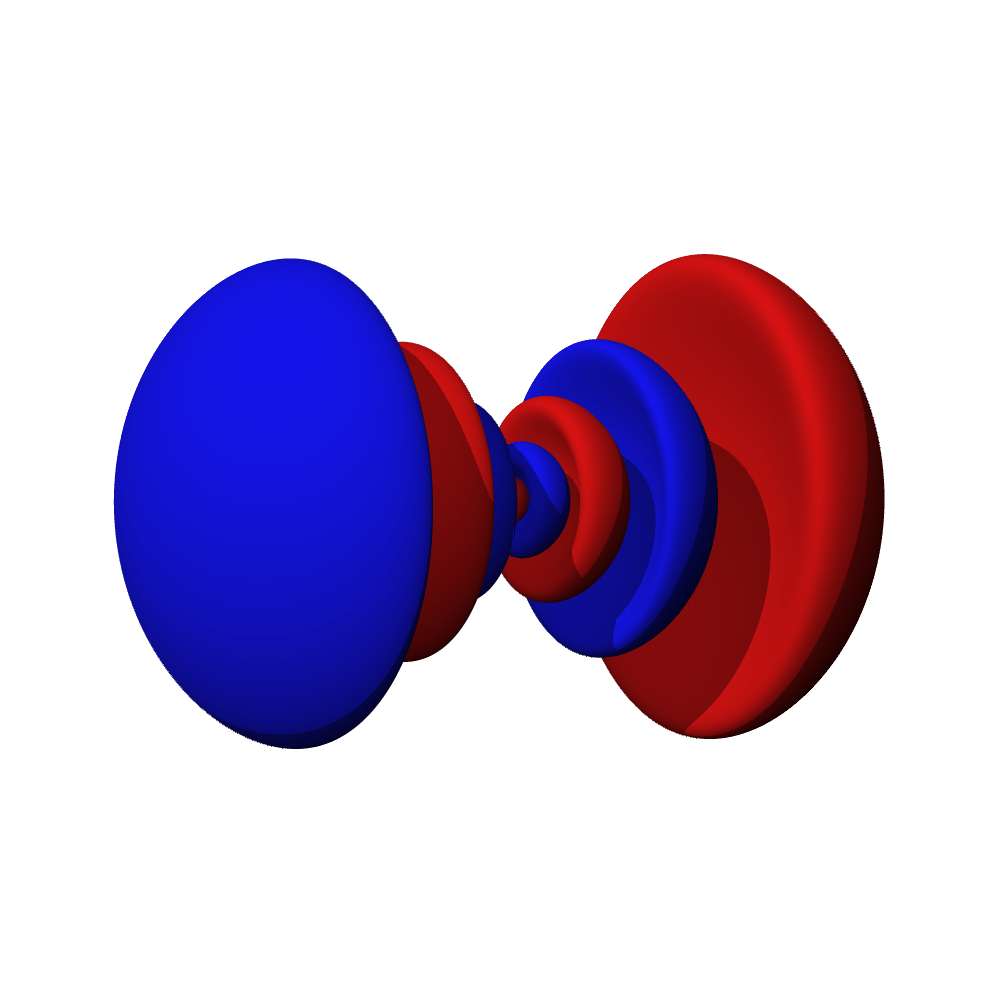
\includegraphics[width=1.6cm]{tableau_geometrie_orbitale_modelisation/P6x.png}  
&
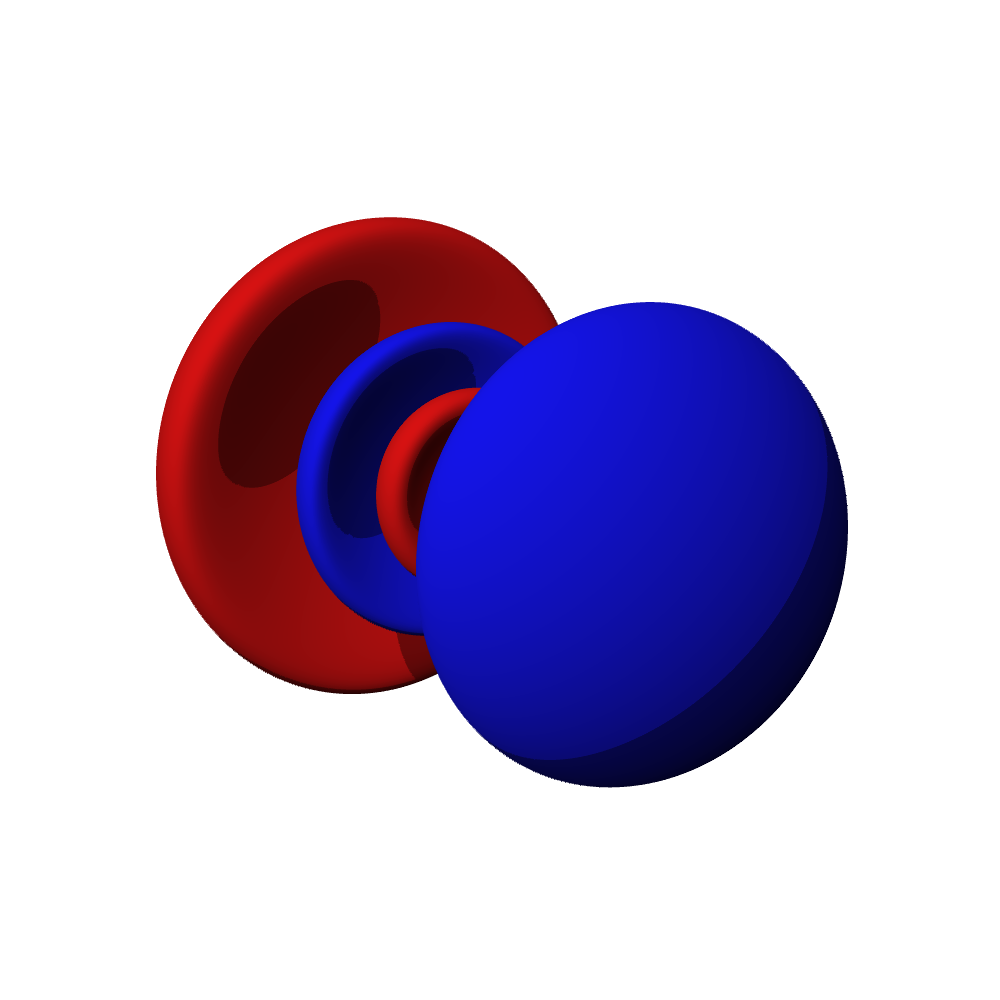
\includegraphics[width=1.6cm]{tableau_geometrie_orbitale_modelisation/P6y.png} 
& & & & \\

& & & \makecell[c]{$6p_z$} & \makecell[c]{$6p_x$} & \makecell[c]{$6p_y$} & & & &  \\ %centrer la cellule individuellement 

\addlinespace

 & \multirow[t]{2}{*}{$\ell=2$} & \multirow[t]{2}{*}{$6d$} & 
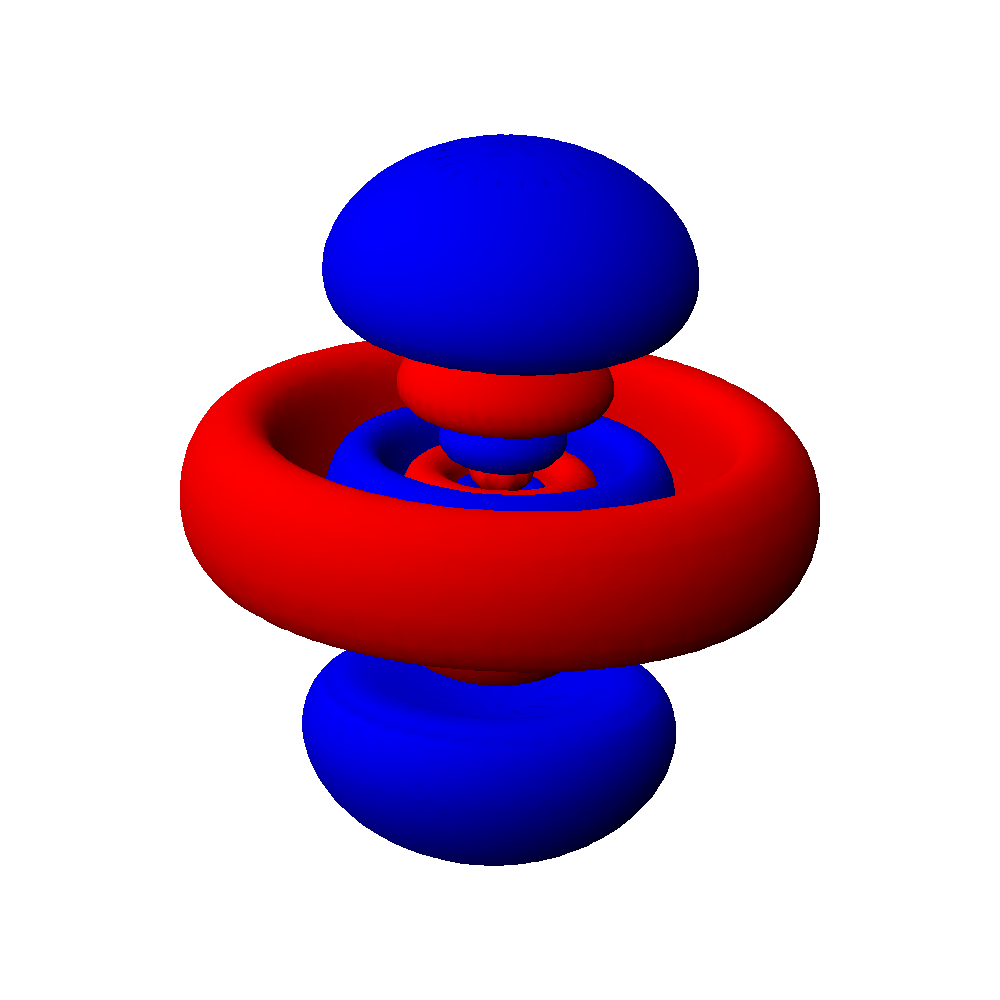
\includegraphics[width=1.6cm]{tableau_geometrie_orbitale_modelisation/D6z2.png} 
&
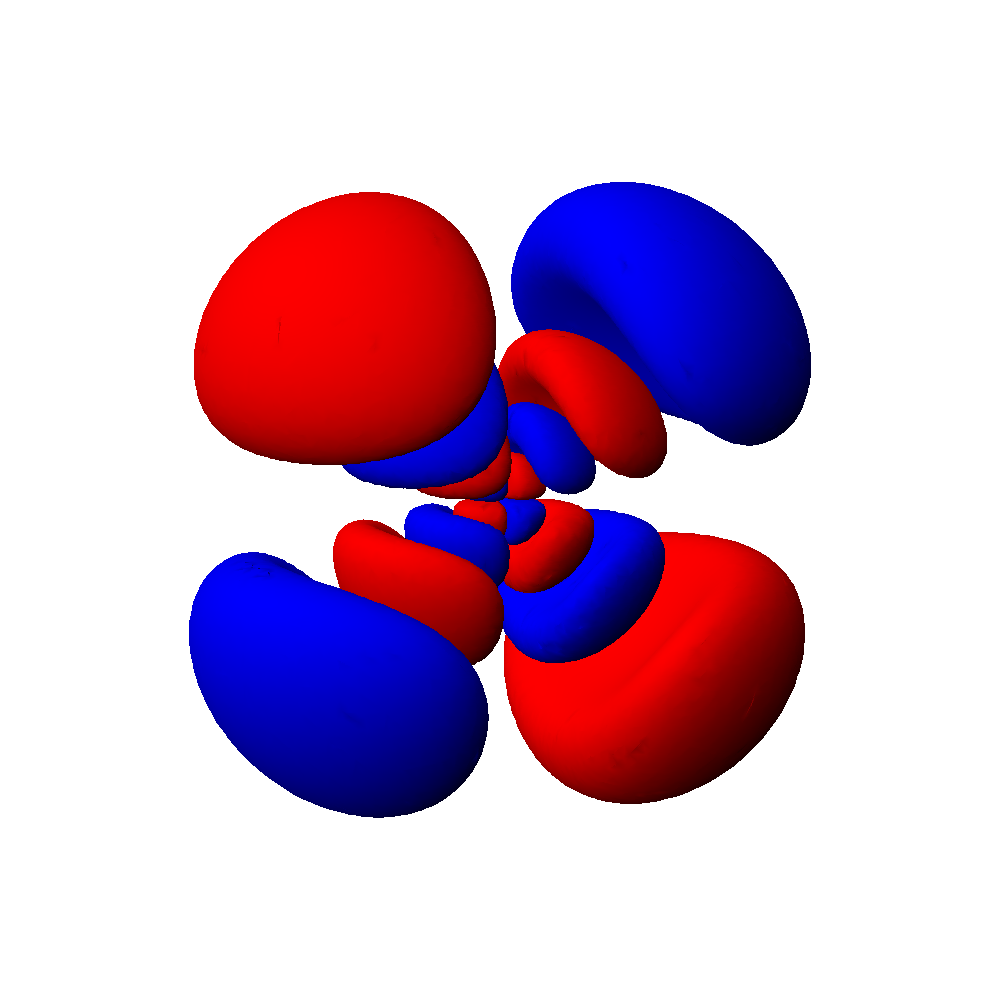
\includegraphics[width=1.6cm]{tableau_geometrie_orbitale_modelisation/D6xz.png}  
&
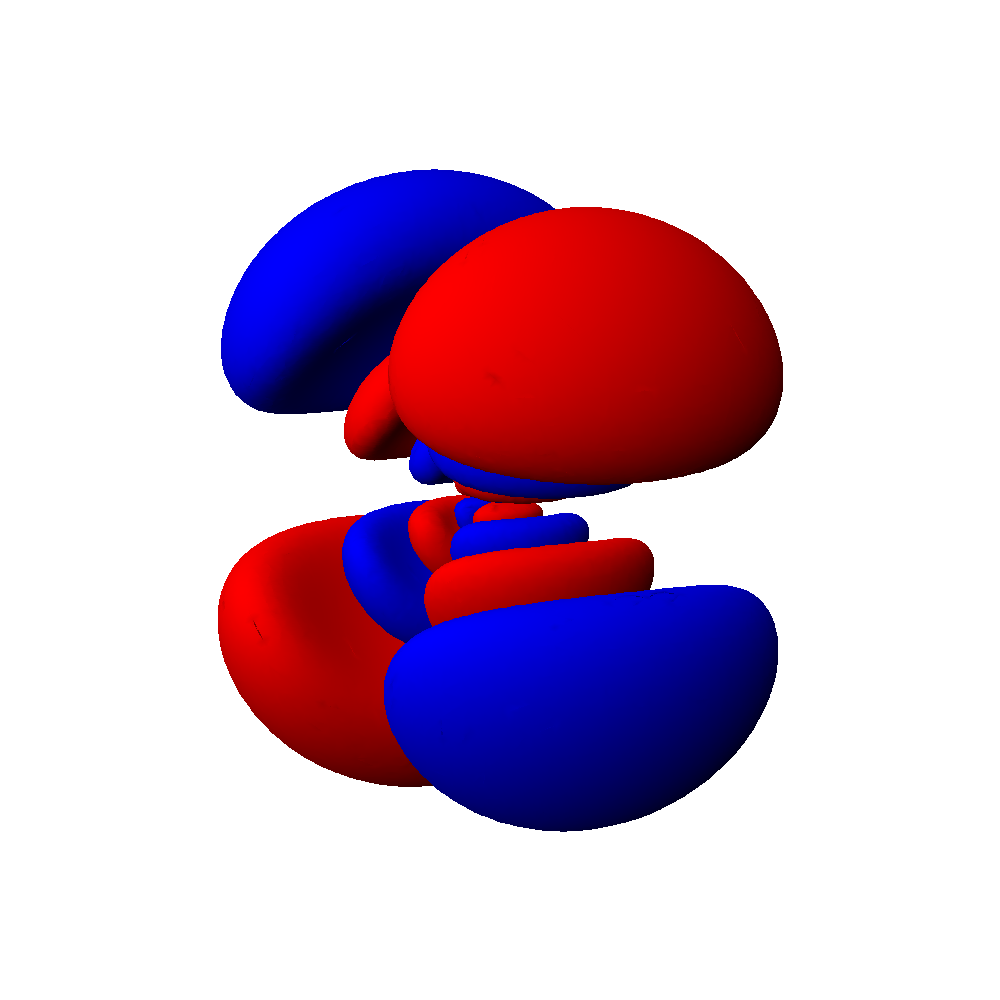
\includegraphics[width=1.6cm]{tableau_geometrie_orbitale_modelisation/D6yz.png} 
& 
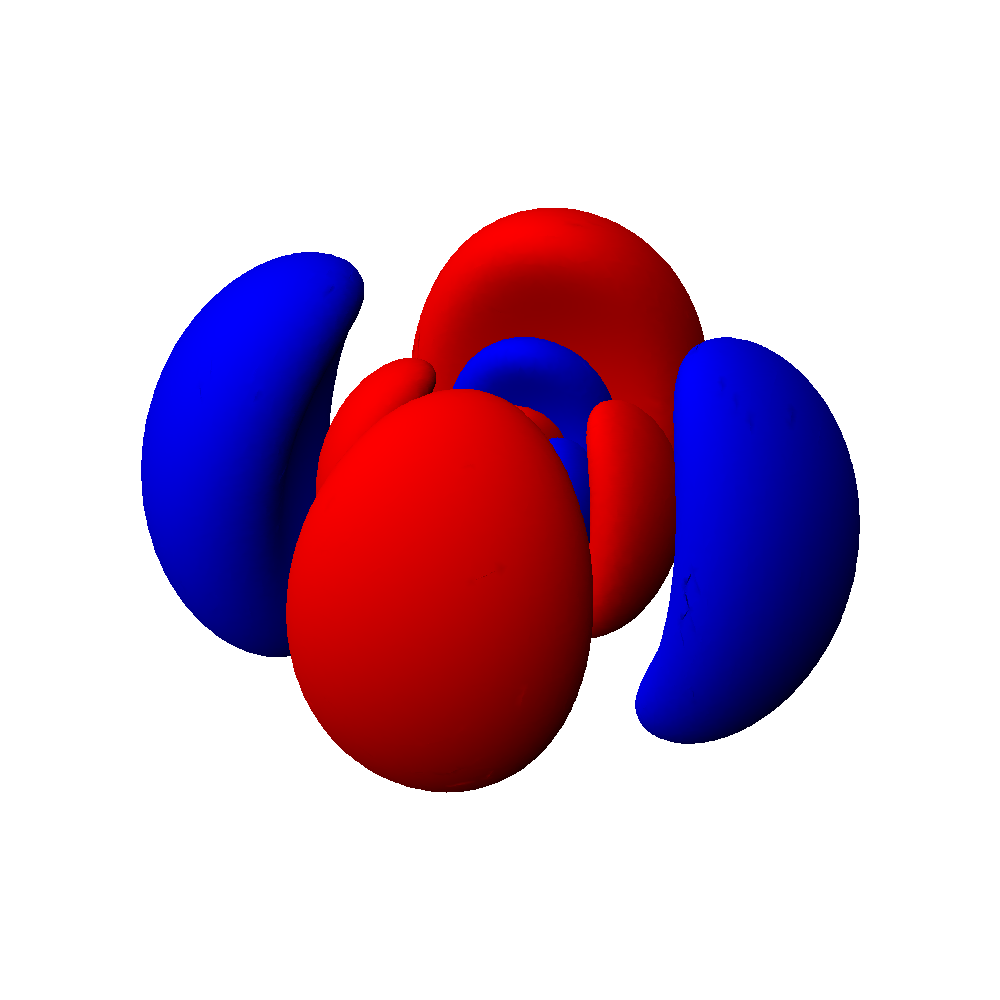
\includegraphics[width=1.6cm]{tableau_geometrie_orbitale_modelisation/D6xy.png} 
&
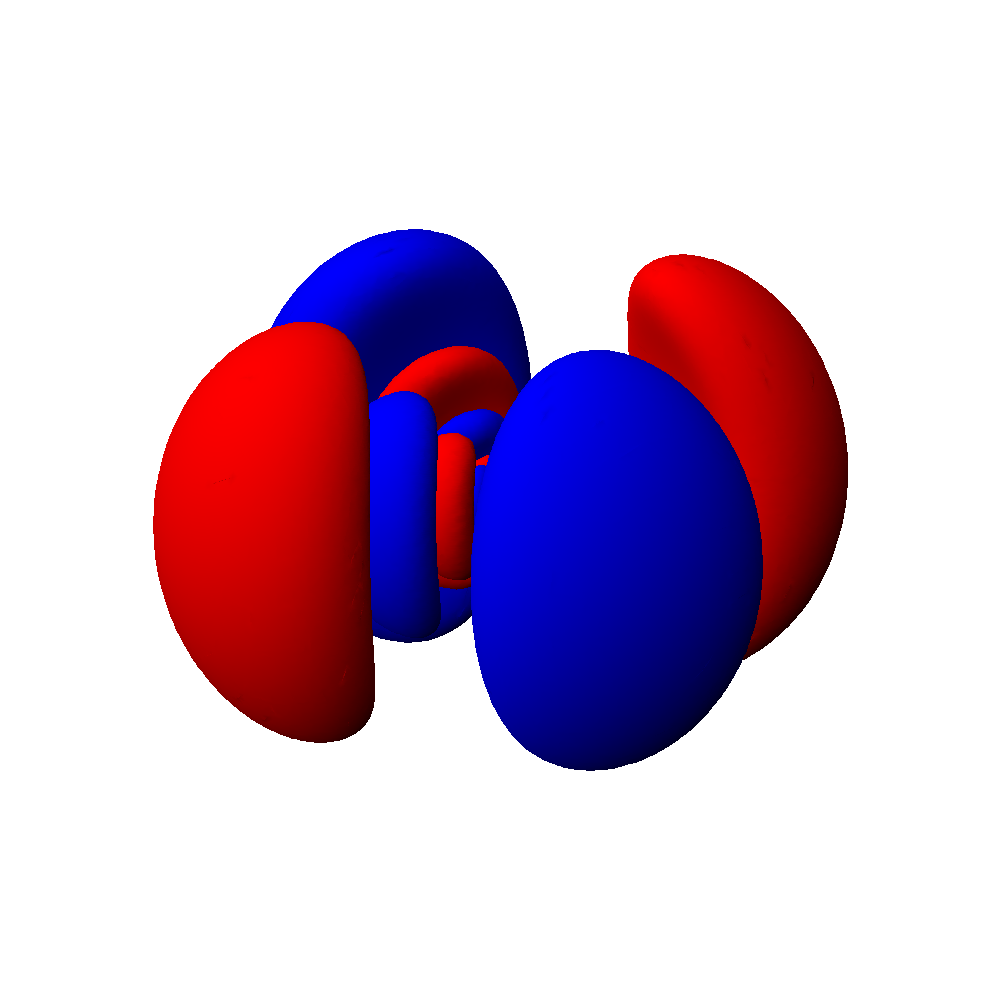
\includegraphics[width=1.6cm]{tableau_geometrie_orbitale_modelisation/D6x2-y2.png} 
& & \\
& & & \makecell[c]{$6d_{z^2}$} & \makecell[c]{$6d_{xz}$} & \makecell[c]{$6d_{yz}$} & \makecell[c]{$6d_{xy}$} & \makecell[c]{$6d_{x^{2}-y^{2}}$} & &  \\ %centrer la cellule individuellement 

\midrule

\multirow[t]{2}{*}{$n=7$} & \multirow[t]{2}{*}{$\ell=0$} & \multirow[t]{2}{*}{$7s$} & 
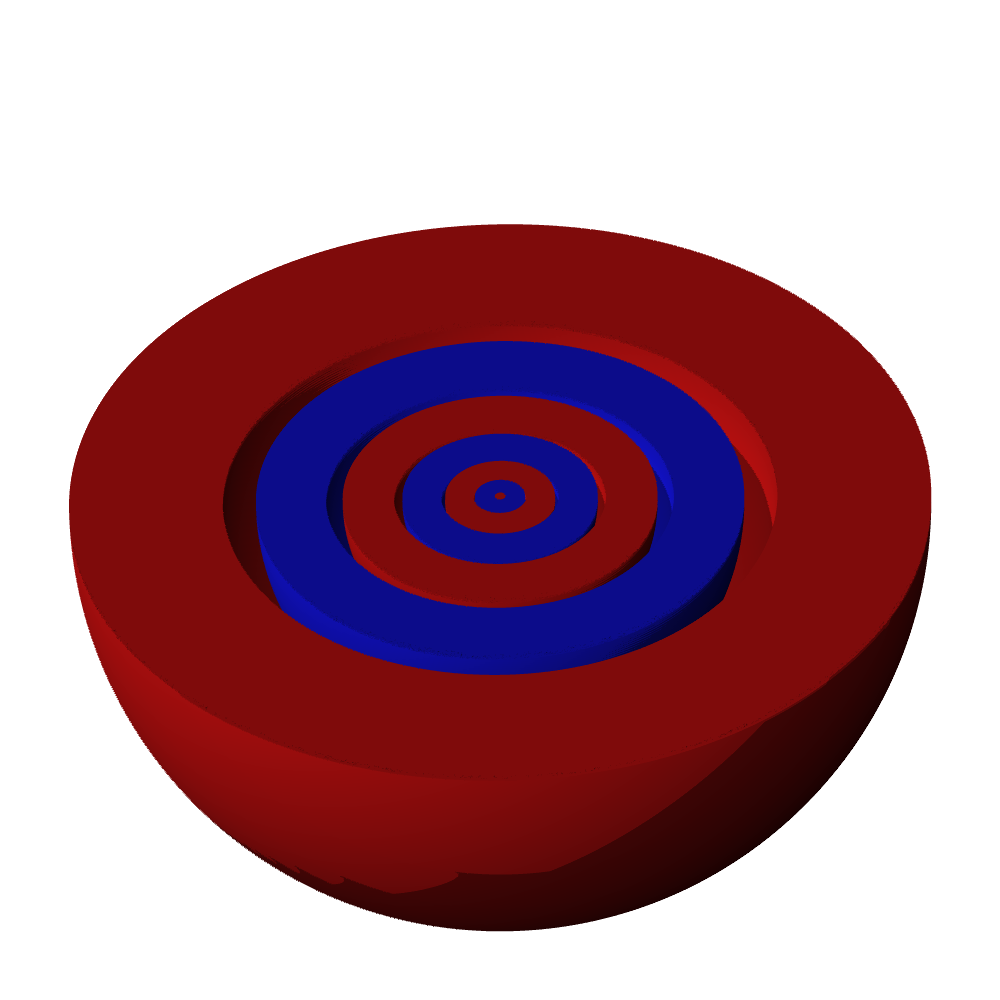
\includegraphics[width=1.6cm]{tableau_geometrie_orbitale_modelisation/S7M0.png} 
& & & & & & \\

& & & \makecell[c]{$7s$} & & & & & &  \\ %centrer la cellule individuellement 

\bottomrule

\end{xltabular}
\end{landscape}

%end{document}


\begin{figure}[!h]
		\centering
		\animategraphics[autoplay, loop, scale=0.8]{10}{fig_aluminium_modelisation_anime}{}{}
		\caption{Modélisation animée d'un atome d'aluminium avec ses différentes couches atomiques}
		\label{fig:aluminium_modelisation_animee}
\end{figure}

%\end{document}